\documentclass[18pt]{beamer}
\usetheme{Madrid}

\usepackage{graphics}
\usepackage{listings}
\usepackage{url}
\usepackage{verbatim}
\usepackage{xcolor}

\lstset{language=C++,numbersep=1pt,identifierstyle=\color{blue!50!black},commentstyle=\color{yellow!50!black},xleftmargin=7pt,numberblanklines=false,numberstyle=\color{red!60!black},numbers=left,basicstyle=\tiny\ttfamily,keywordstyle=\color{green!60!black}\bfseries,stringstyle=\color{red!80!black}}

\newcommand{\lstlistingwithnumber}[3]{
\begin{center}
\lstinputlisting[linerange={#1-#2},firstnumber=#1]{#3}
\end{center}
}

\newcommand{\centeredlargetext}[3]{
{
\setbeamertemplate{background}{}
\setbeamertemplate{navigation symbols}{}
\setbeamercolor{background canvas}{bg={#1}}
\color{#2}
\begin{frame}[plain]
\fontsize{36pt}{36pt}\selectfont
\center
\begin{center}
{#3}
\end{center}
\end{frame}
}}

\newcommand{\centeredhugetext}[3]{
{
\setbeamertemplate{navigation symbols}{}
\setbeamercolor{background canvas}{bg={#1}}
\fontsize{72pt}{72pt}\selectfont
\color{#2}
\begin{frame}[plain]
\center
\begin{center}
{#3}
\end{center}
\end{frame}
}}


\begin{document}

\title[ITKv4]{ITKv4 - The Next Generation}
\subtitle[ITKv4]{What is new in ITKv4}
\institute[Insight Software Consortium]{Insight Software Consortium}
\date[May 2012]{May 2012}

\begin{frame}
\titlepage
\end{frame}


{
\setbeamertemplate{navigation symbols}{}
\begin{frame}[plain]
\center
\begin{center}
This presentation is copyrighted by\\
The \textbf{Insight Software Consortium}\\
\bigskip
distributed under the\\
\textbf{Creative Commons by Attribution License 3.0}\\
\url{http://creativecommons.org/licenses/by/3.0}\\
\end{center}
\end{frame}
}


\begin{frame}
  \tableofcontents[hideallsubsections]
\end{frame}

\setbeamertemplate{background}{
\includegraphics[width=\paperwidth]{../Art/ITKv4_transparent}}

\section{Virtual Machines Preparation}

\centeredlargetext{white}{black}{
Virtual Machines Preparation
}

\begin{frame}
\frametitle{Virtual Machines Preparation}
\begin{itemize}
\item Get DVD / USB Memory Stick
\item Install VirtualBox from it
\item Import the VirtualMachine file
\item Boot the Virtual Machine
\item Log in
\item Get familiar with directories
\end{itemize}
\end{frame}


\begin{frame}
\frametitle{Media Content}
\framesubtitle{Directories and Files}
\begin{itemize}
\item VirtualBoxInstallers
\begin{itemize}
\item VirtualBox-4.0.8-71778-OSX.dmg (Mac)
\item VirtualBox-4.0.8-71778-Win.exe (Windows)
\item (Ubuntu Linux)
\begin{itemize}
\item virtualbox-4.0\_4.0.8-71778~Ubuntu~lucid\_amd64.deb
\item virtualbox-4.0\_4.0.8-71778~Ubuntu~lucid\_i386.deb
\item virtualbox-4.0\_4.0.8-71778~Ubuntu~maverick\_amd64.deb
\item virtualbox-4.0\_4.0.8-71778~Ubuntu~maverick\_i386.deb
\item virtualbox-4.0\_4.0.8-71778~Ubuntu~natty\_amd64.deb
\item virtualbox-4.0\_4.0.8-71778~Ubuntu~natty\_i386.deb
\item \ldots
\end{itemize}
\end{itemize}
\pause
\item VirtualMachine
\begin{itemize}
\item  OpenCV-ITK-disk1.vmdk
\item  OpenCV-ITK.ovf
\end{itemize}
\end{itemize}
\end{frame}

\begin{frame}
\frametitle{Install VirtualBox}
\begin{itemize}
\item Select the installer for your platform
\item Run it
\end{itemize}
\end{frame}

\begin{frame}
\frametitle{Alternative Linux Installation}
\begin{itemize}
\item  You can also install VirtualBox by doing:
\item  sudo apt-get install virtualbox-ose-qt
\end{itemize}
\end{frame}

\begin{frame}
\frametitle{Importing the Virtual Machine}
\begin{itemize}
\item Run VirtualBox
\item In ``File'' Menu select ``Import Appliance''
\item Provide the filename in the DVD / USB stick ``VirtualMachine/OpenCV-ITK.ovf"
\item A progress bar will appear, and when it finishes you should see:
\end{itemize}
\begin{center}
  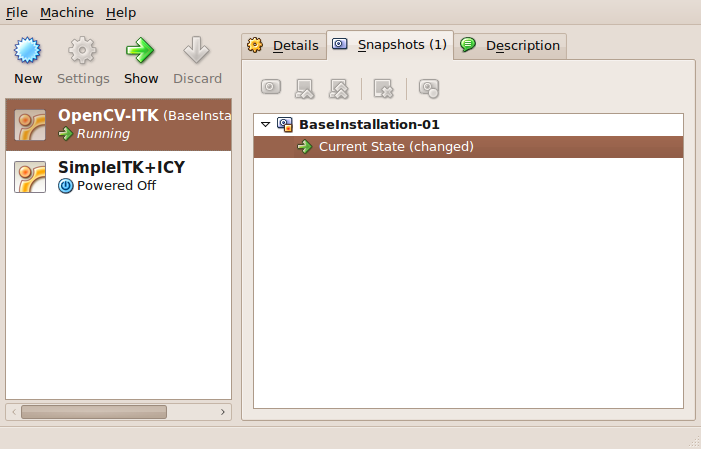
\includegraphics[width=0.5\paperwidth]{Screenshot-VirtualBox-OSE-01.png}
\end{center}
\end{frame}


\centeredlargetext{white}{black}{
We will get back...
}


\centeredlargetext{black}{white}{
ITKv4
}

\section{Overview}

\centeredlargetext{white}{black}{
Overview
}

\centeredlargetext{white}{black}{
10 Years Old
}

\centeredlargetext{white}{black}{
\$ 5 Million
}

\centeredlargetext{white}{black}{
ARRA Funds
}

\centeredlargetext{white}{black}{
1.5 Years
}

\centeredlargetext{white}{black}{
Next 10 Years
}

\begin{frame}
\frametitle{ITKv4 Team}
\large
\begin{itemize}
\item GE Global Research
\pause
\item Kitware Inc.
\pause
\item Harvard University
\pause
\item Mayo Clinic
\pause
\item University of Iowa
\pause
\item University of Pennsylvania
\pause
\item CoSMo Software
\pause
\item National Library of Medicine
\end{itemize}
\end{frame}

\begin{frame}
\frametitle{A2D2 Team}
\large
\begin{itemize}
\item Georgetown University
\pause
\item University of Utah
\pause
\item UNC - Chape Hill
\pause
\item The Ohio State University
\pause
\item Old Dominion University
\pause
\item Carnegie Mellon University
\pause
\item Harvard University
\pause
\item University of Utah
\pause
\item William and Mary
\pause
\item Kitware Inc.
\pause
\item Cornell University
\end{itemize}
\end{frame}

\centeredlargetext{white}{black}{
Major Changes
}


\centeredlargetext{black}{white}{
Apache 2.0 License
}

\centeredlargetext{black}{white}{
``Patented''\\
Directory\\
Removed
}


\centeredlargetext{black}{white}{
New\\
Software Process
}

\begin{frame}
\frametitle{Software Process}
\Huge
\begin{itemize}
\item Git
\pause
\item Gerrit
\pause
\item cdash@home
\pause
\item Improved Testing Data
\end{itemize}
\end{frame}


{
\setbeamertemplate{navigation symbols}{}
\begin{frame}
  \frametitle{Code Review}
  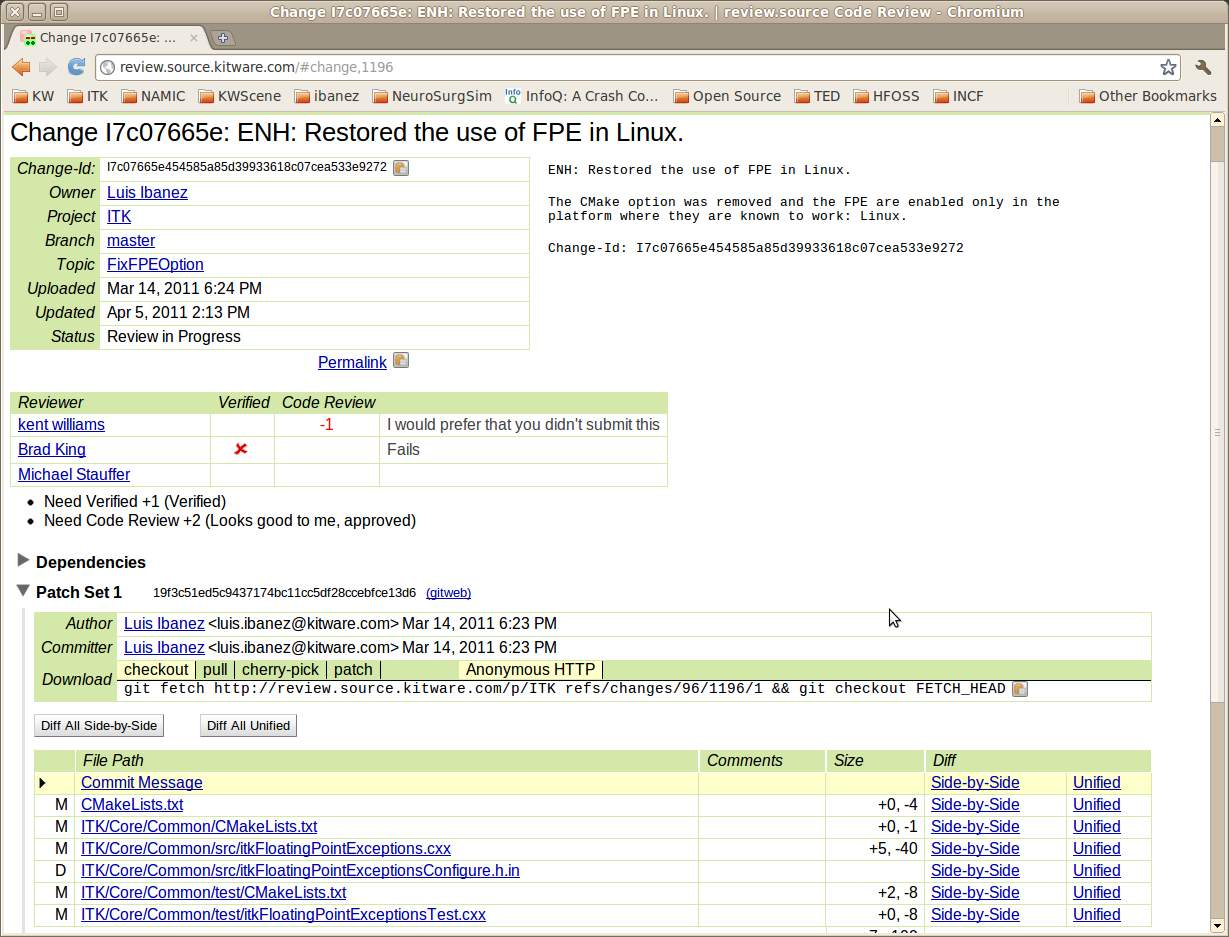
\includegraphics[width=\textwidth,height=\paperheight]{../Art/ITKGerritScreenShot.jpg}
\end{frame}
}


\centeredlargetext{black}{white}{
Modern C++
}


\begin{frame}
\frametitle{Deprecated Compilers}
\Huge
\begin{itemize}
\item Visual Studio 6.0, 7.0
\pause
\item Borland 5.5
\pause
\item Sun CC $<$ 5.9
\pause
\item SGI CC
\pause
\item MWORKS
\pause
\item Cygwin
\pause
\item GCC $<$ 3.4
\end{itemize}
\end{frame}



\centeredlargetext{black}{white}{
64 Bits
}


\begin{frame}
\frametitle{64 Bits}
\Huge
\begin{itemize}
\item Since 2008
\pause
\item In Windows 64bits:\\unsigned long is 32bits
\pause
\item Use typedef !
\pause
\item ITK\_USE\_64BITS\_IDS
\end{itemize}
\end{frame}


\begin{frame}
\frametitle{ITK Libraries}
\Huge
\begin{itemize}
\item ITKCommon, ITKIO, ITKImageIntensity, $\cdots$
\pause
\item is now:
\pause
\item \$\{ITK\_LIBRARIES\}
\end{itemize}
\end{frame}




\section{Virtual Machines Preparation II}

\centeredlargetext{white}{black}{
Virtual Machine Preparation II
}

\subsection{Booting the Virtual Machine}
\begin{frame}
\frametitle{Booting the Virtual Machine}
\begin{itemize}
\item Click on the ``ITKv4'' icon on the left, to select it.
\item Click on the Green Arrow at the top ``Show''.
\item The VM will start to boot and you will see the warning:
\end{itemize}
\begin{center}
  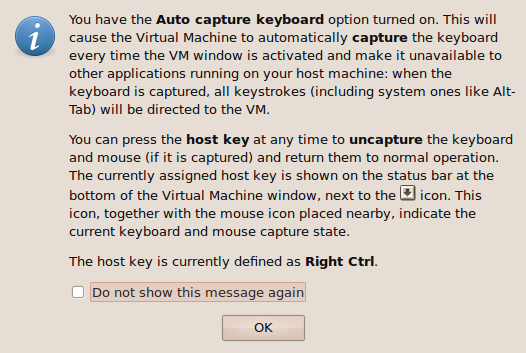
\includegraphics[width=0.4\paperwidth]{../Art/Screenshot-VirtualBox-OSE-02.png}
\end{center}
\begin{itemize}
\item Click ``OK''
\end{itemize}
\end{frame}

\begin{frame}
\frametitle{Booting the Virtual Machine}
\begin{itemize}
\item The boot sequence should continue and you should see:
\end{itemize}
\begin{center}
  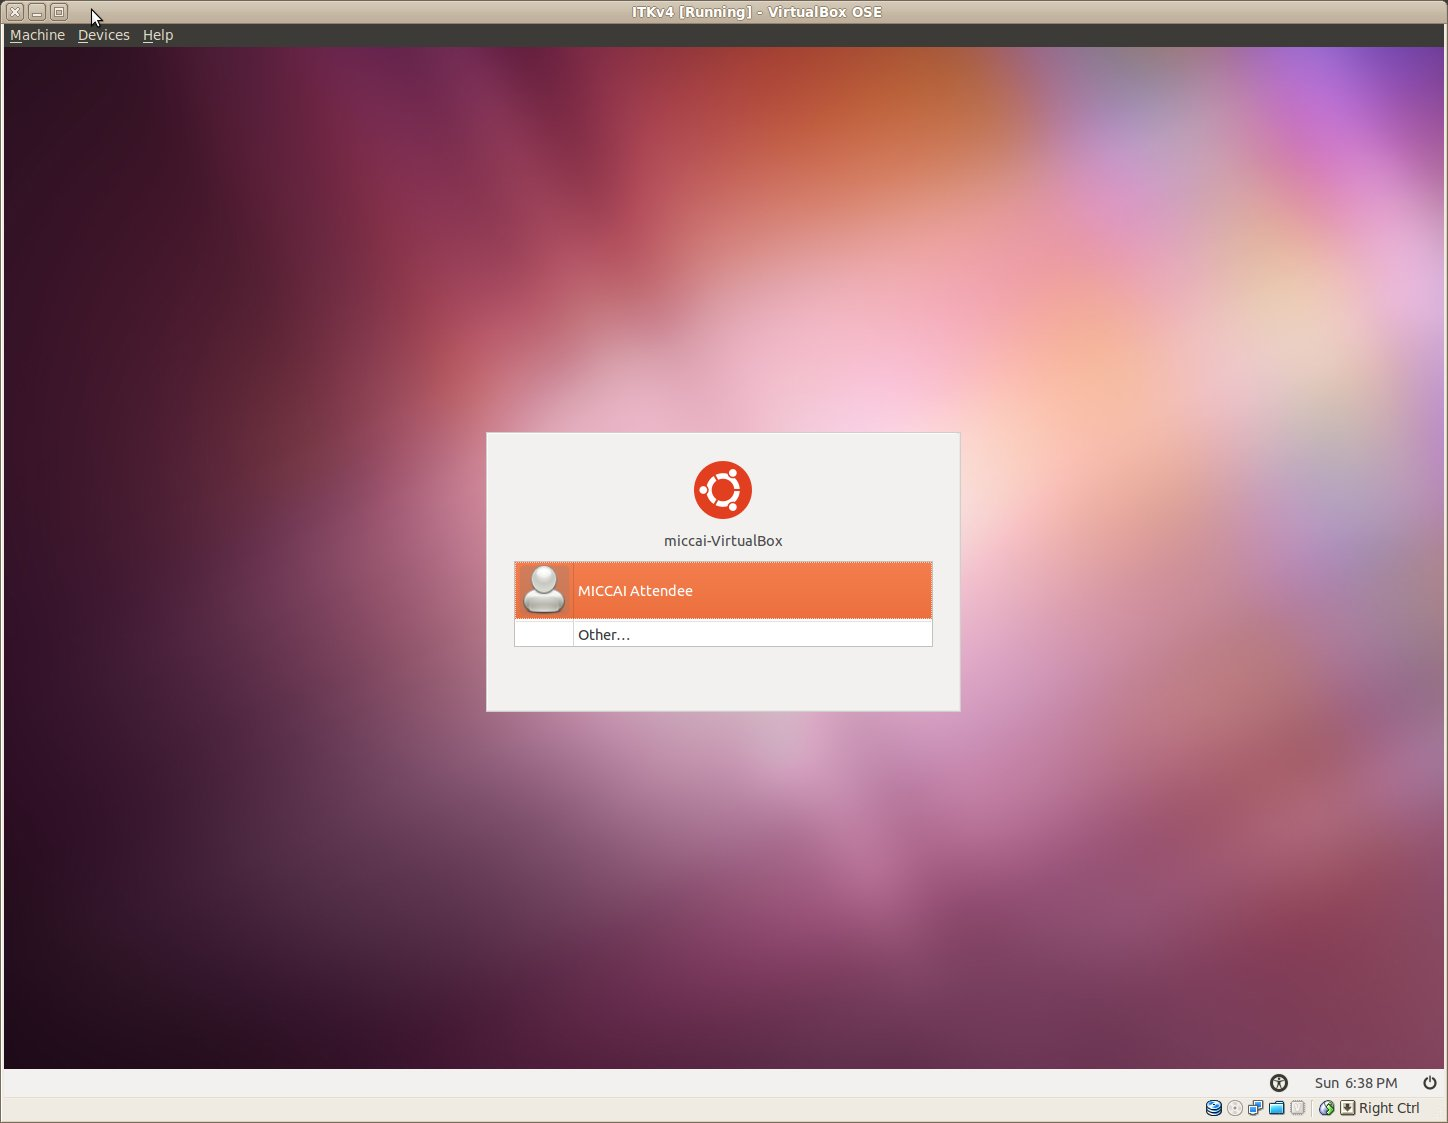
\includegraphics[width=0.7\paperwidth]{../Art/Screenshot-ITKv4-VirtualBox-01.jpg}
\end{center}
\begin{itemize}
\item Login with the password: ``toronto''
\end{itemize}
\end{frame}

\begin{frame}
\frametitle{Booting the Virtual Machine}
\begin{itemize}
\item After logging in you should see:
\end{itemize}
\begin{center}
  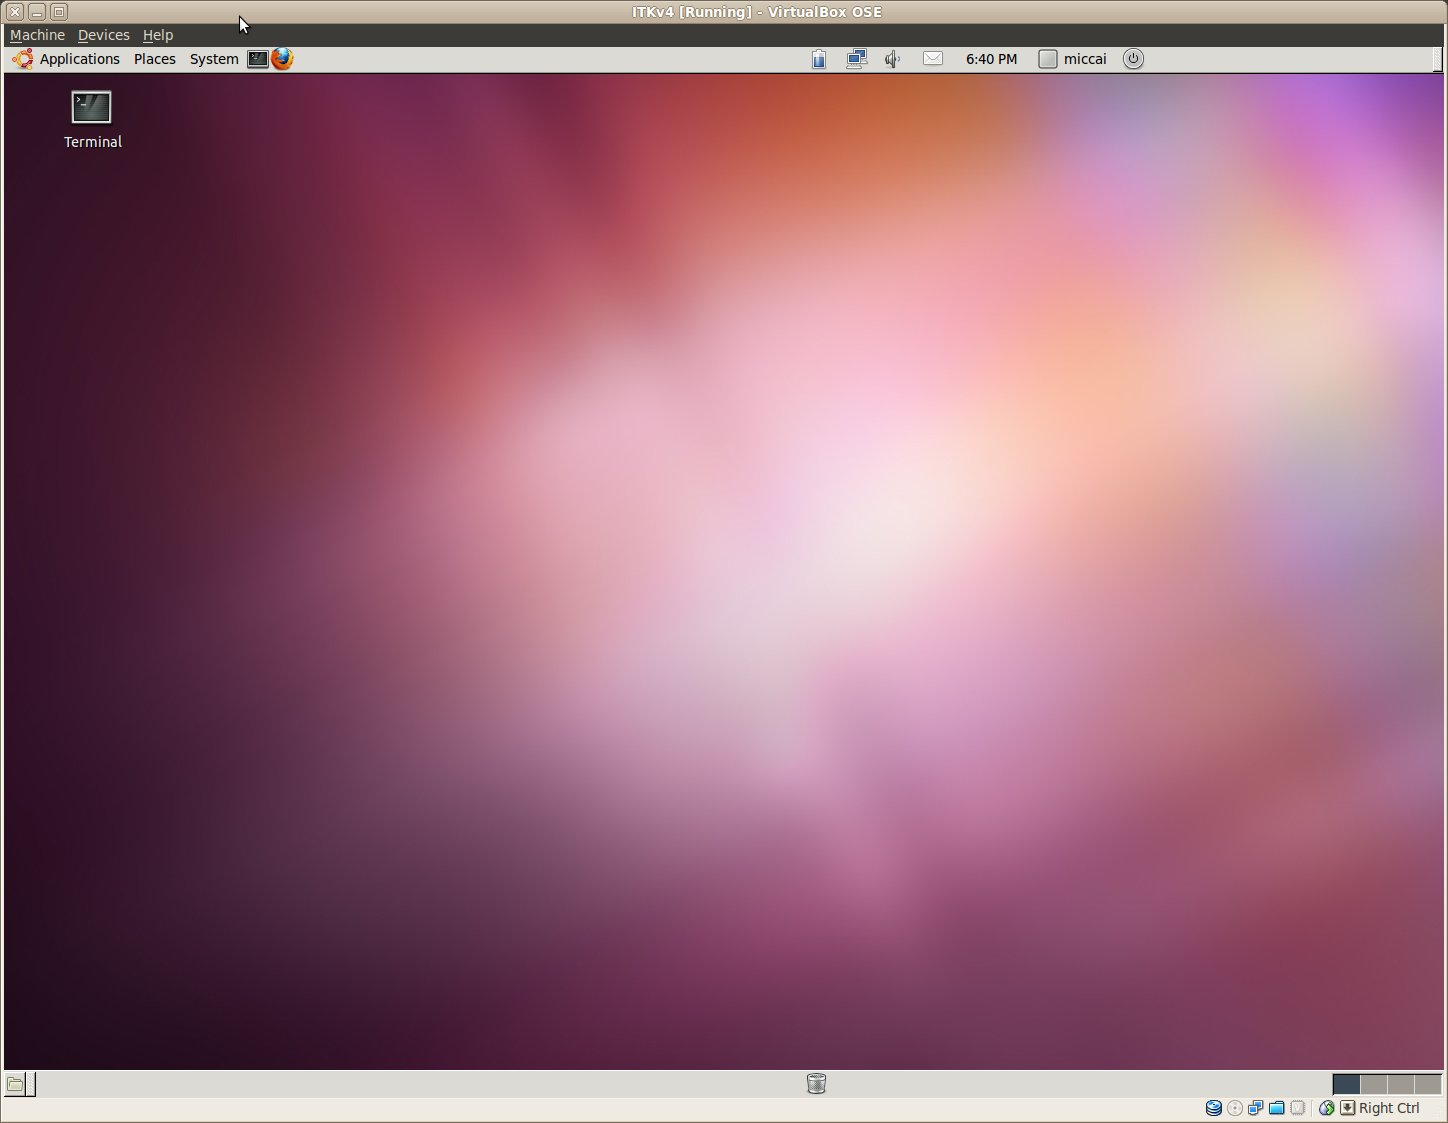
\includegraphics[width=0.7\paperwidth]{../Art/Screenshot-ITKv4-VirtualBox-02.jpg}
\end{center}
\end{frame}


\centeredlargetext{white}{black}{
Your Virtual Machine\\ is Ready !
}

\begin{frame}
\frametitle{Additional Copies}
\begin{itemize}
\item The same source trees are available in the DVD / USB key
\item Outside of the VirtualBox image
\end{itemize}
\end{frame}



\subsection{Software Environment}

\centeredlargetext{white}{black}{
Software Environment
}

{
\setbeamertemplate{background}{}
\begin{frame}
\frametitle{Welcome to Debian GNU/Linux}
\begin{center}

\includegraphics[height=0.5\paperheight]{../Art/Tux.png}
%
\includegraphics[width=0.5\paperwidth]{../Art/blackeubuntulogo.png}
\end{center}
\end{frame}
}

{
\setbeamertemplate{background}{}
\begin{frame}
\frametitle{How to take the mouse out of the Virtual Machine}
\begin{itemize}
\item Hit the \textbf{RIGHT CTRL} Key on Windows / Linux Host
\item Hit the \textbf{LEFT APPLE} Key on Mac Host
\end{itemize}
\end{frame}
}

{
\setbeamertemplate{background}{}
\begin{frame}
\frametitle{How to Open a Terminal - Menu in Lower Left Corner}
\framesubtitle{To type your command line instructions}
\begin{center}
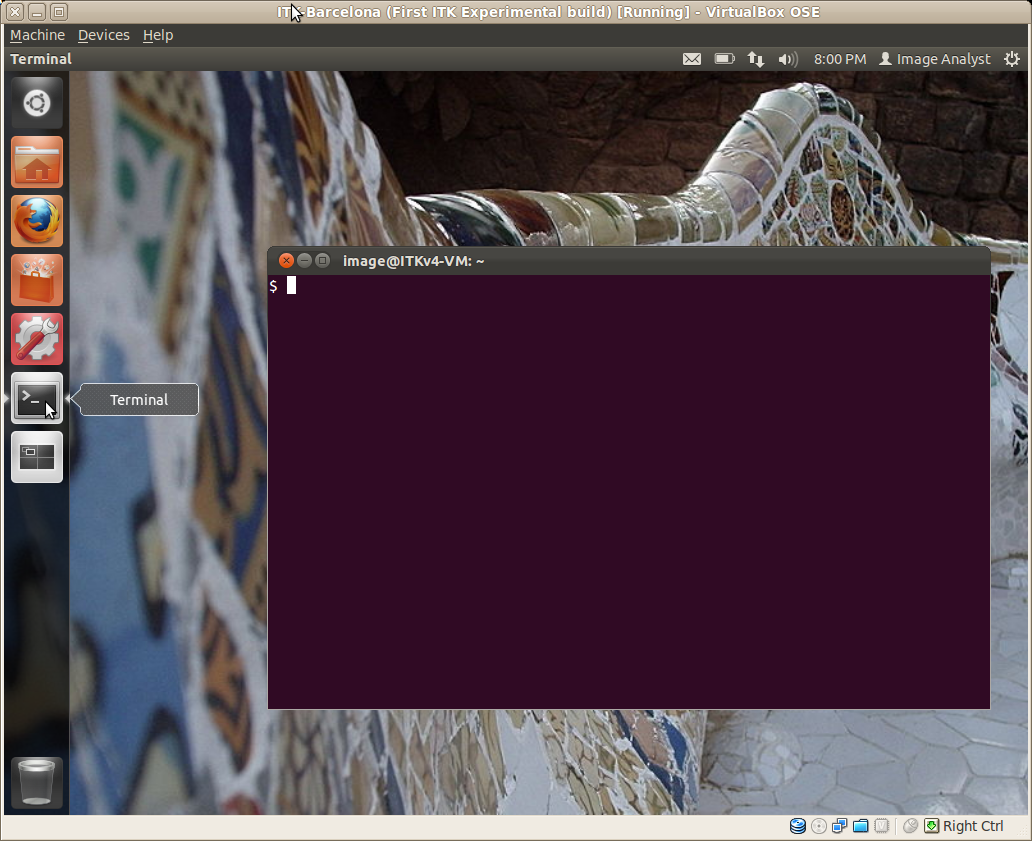
\includegraphics[width=0.7\paperwidth]{../Art/Screenshot-OpenTerminal.jpg}
\end{center}
\end{frame}
}

{
\setbeamertemplate{background}{}
\begin{frame}
\frametitle{How to Navigate Directories}
\framesubtitle{Double Click in Folder Icons in the Desktop}
\begin{center}
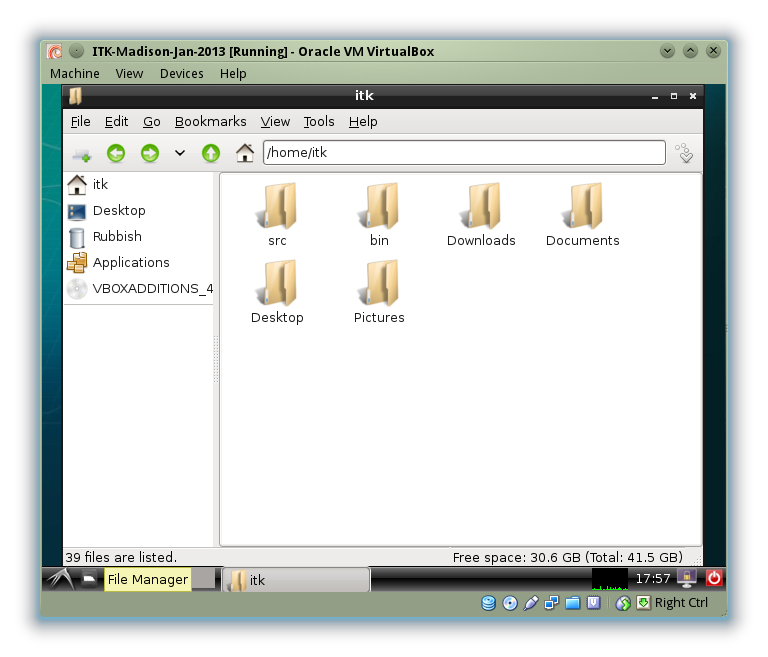
\includegraphics[width=0.7\paperwidth]{../Art/Screenshot-PCManFM.png}
\end{center}
\end{frame}
}

{
\setbeamertemplate{background}{}
\begin{frame}[fragile]
\frametitle{Walk through the directories}
\begin{itemize}
\item Find source code of exercises
\begin{verbatim}
cd ~/src/ITKv4-TheNextGeneration-Tutorial/Exercises
pwd
ls
pcmanfm .
\end{verbatim}
\pause
\item Find binary build of exercises
\begin{verbatim}
cd ~/bin/ITKv4-TheNextGeneration-Tutorial/Exercises
pwd
ls
\end{verbatim}
\end{itemize}
\end{frame}
}

{
\setbeamertemplate{background}{}
\begin{frame}[fragile]
\frametitle{The TAB Key is your Friend}
\begin{itemize}
\item When writing filenames
\item Use the TAB key for completions
\item No need to type full filenames
\end{itemize}
\end{frame}
}

{
\setbeamertemplate{background}{}
\begin{frame}[fragile]
\frametitle{How to View Images}
\begin{itemize}
\item Go to the directory
\item Invoke ``ImageViewer'' application
\begin{verbatim}
cd ~/data
ImageViewer BrainProtonDensitySlice.png
\end{verbatim}
\pause
\item Hit ``+'' key to zoom in
\pause
\item Hit ``-'' key to zoom out
\pause
\item Hit ESC key to quit the application
\end{itemize}
\end{frame}
}


\centeredlargetext{black}{white}{
Modularization
}

\section{Modularization}

% -----------------------------------
\subsection{Modularization Motivation}

\begin{frame}
\frametitle{Why Modularization}
\begin{itemize}
\item Growth management
\pause
\item Software quality improvement
\pause
\item Facilitating add-ons
\pause
\item Separate third party libraries
\pause
\item Optional Components
\end{itemize}
\end{frame}

% -----------------------------------
\subsection{Modularization Implementation}

\begin{frame}
\frametitle{Module sizes}
\center
\begin{center}
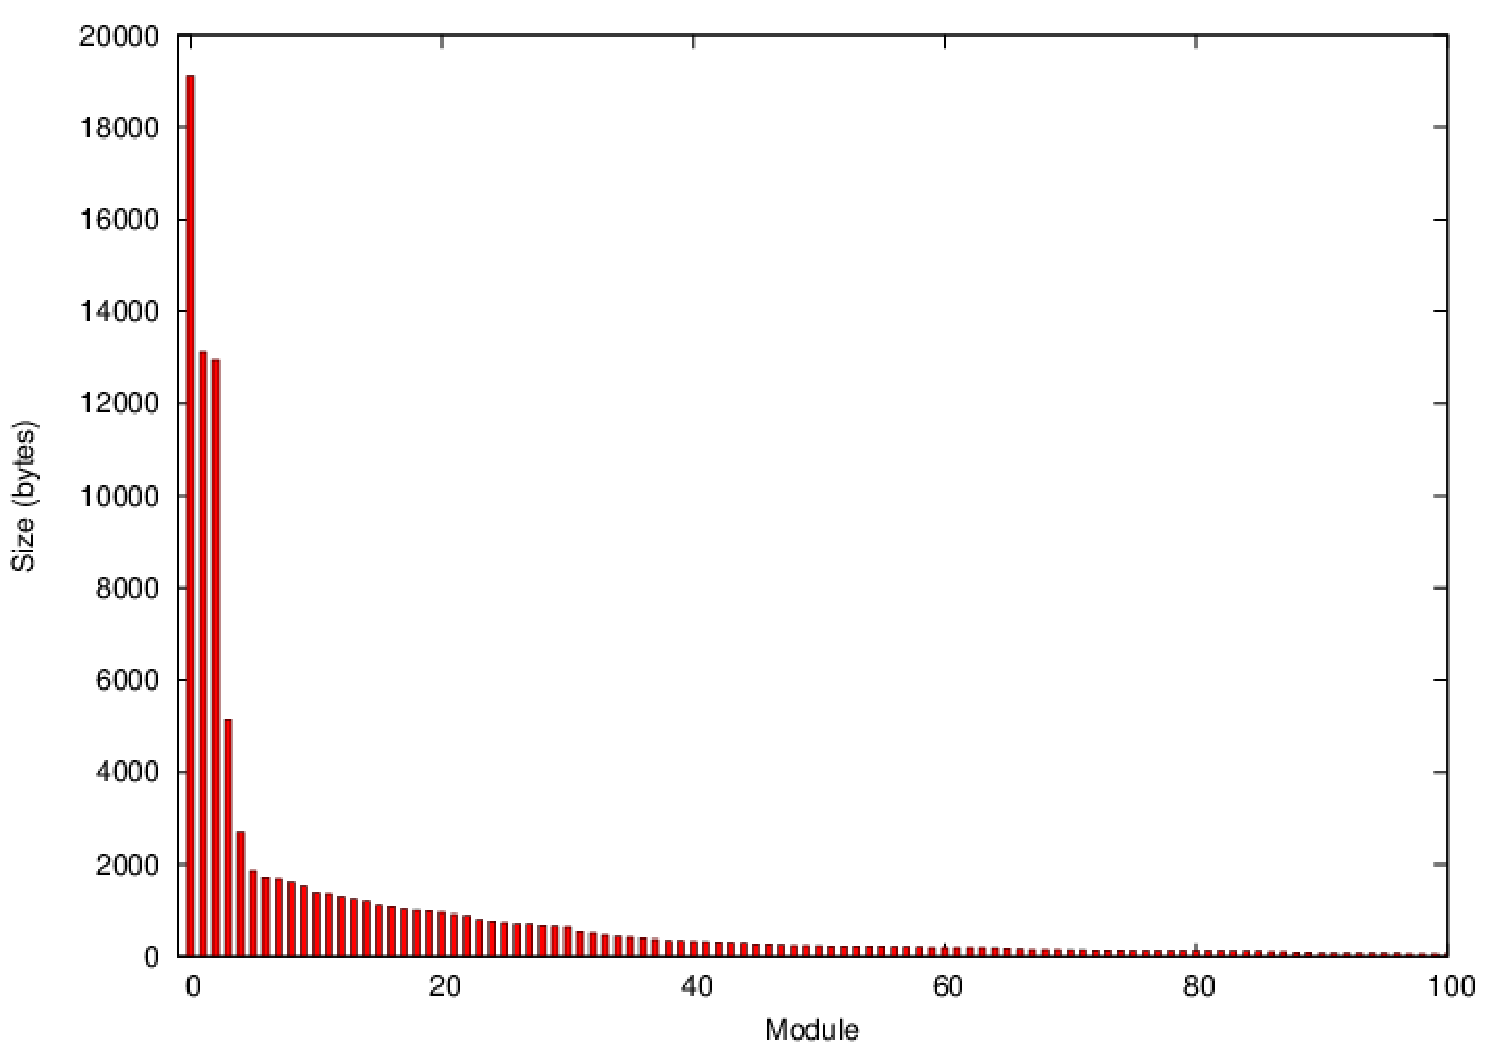
\includegraphics[height=0.8\textheight]{../Art/moduleSizePlot.pdf}
\end{center}
\end{frame}

\begin{frame}
\frametitle{Module sizes (no third party modules)}
\center
\begin{center}
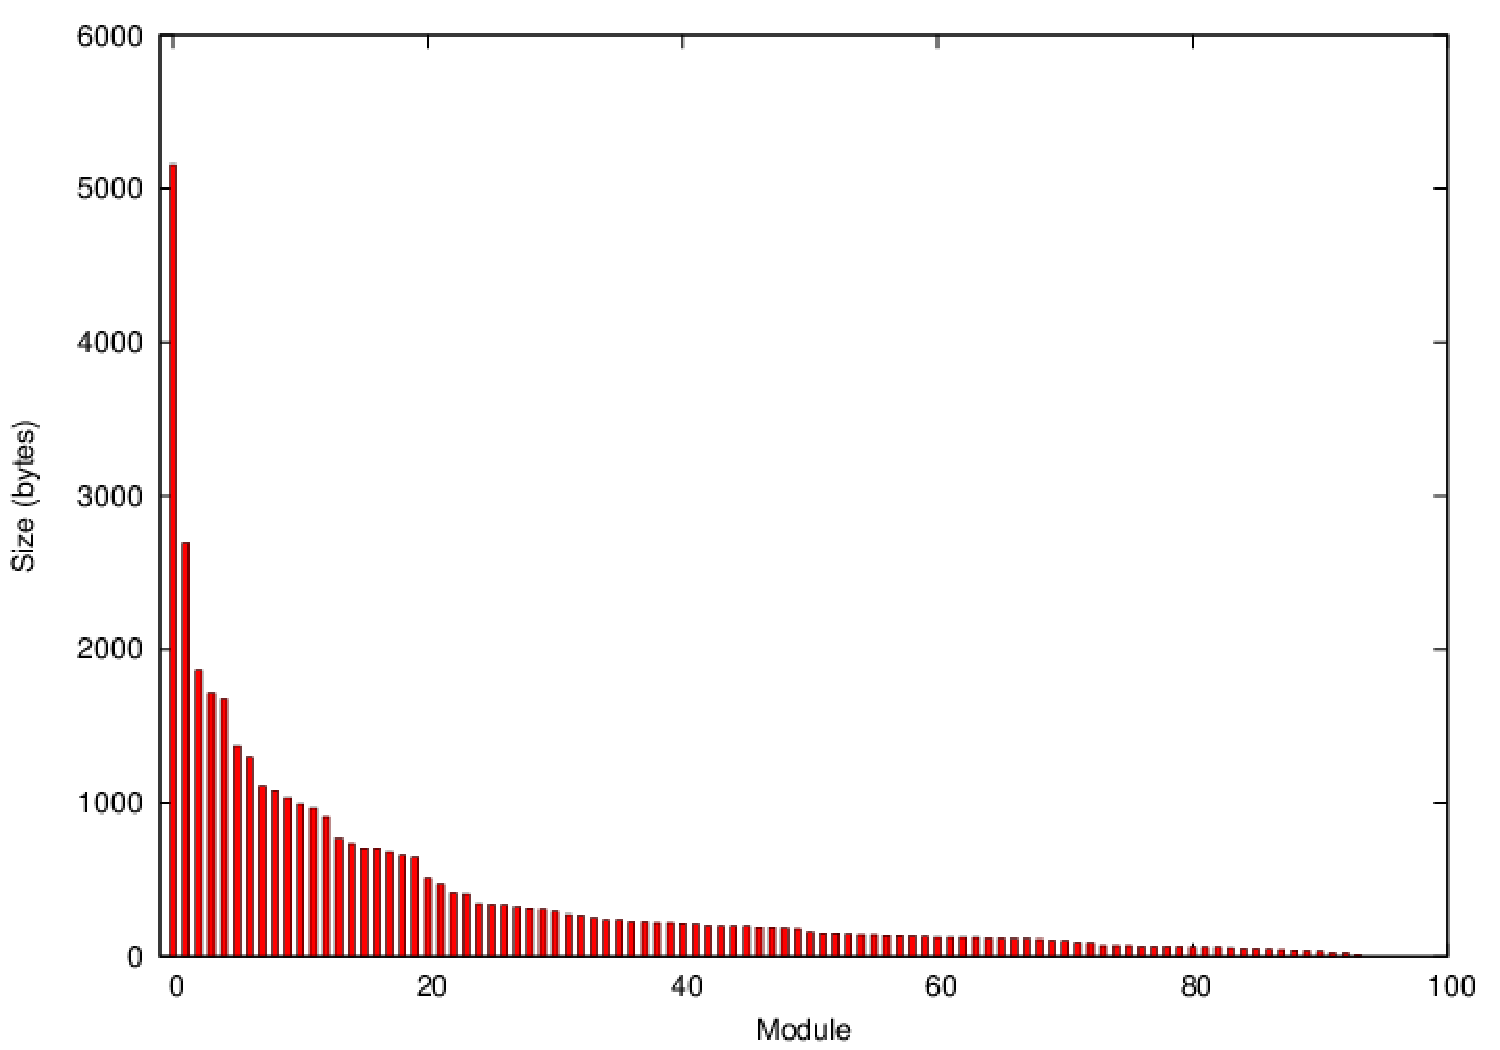
\includegraphics[height=0.8\textheight]{../Art/moduleSizePlotNoThirdParty.pdf}
\end{center}
\end{frame}

\begin{frame}
\frametitle{Visualize dependencies among modules}
\center
\begin{center}
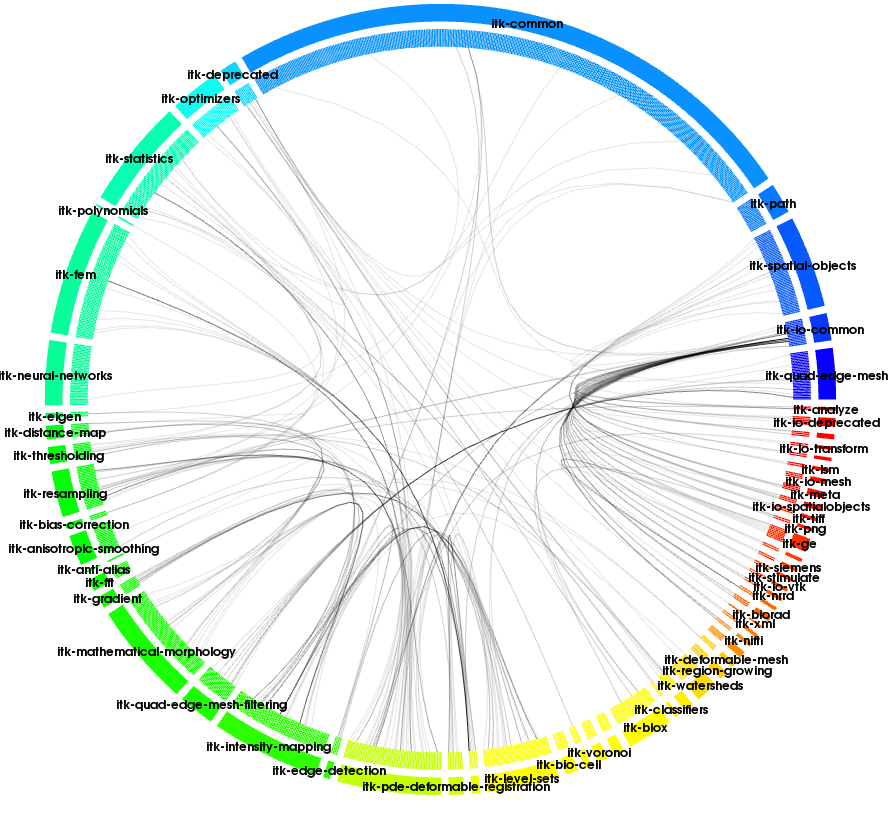
\includegraphics[height=0.8\textheight]{../Art/moduleDependency.png}
\end{center}
\end{frame}

\begin{frame}
\frametitle{ITK Module Grouping}
\begin{itemize}
\item  12 groups, 110 modules and counting
\pause
\item  Group by module functionalities
\pause
\end{itemize}
%\begin{block}
\begin{tabular}{llll}
Bridge     &    \alert{External}   & IO        & Registration \\
Compatibility  & Filtering  & Nonunit   & Segmentation \\
Core           & GPU        & Numerics  & ThirdParty \\
\end{tabular}
%\end{block}
\end{frame}

% -----------------------------------
\subsection{Add Your Own Module}

\begin{frame}
\frametitle{How to add a module into ITK}
\begin{itemize}
\item Where to put a module (categorization)
\pause
\item How to construct a module (CMake magic)
\end{itemize}
\end{frame}


\begin{frame}
\frametitle{Modularization checklist}
\begin{itemize}
\item  Module categorization: module group, module name
\pause
\item  Directory hierarchy: \alert{include}, \alert{test}, \alert{src}
\pause
\item  CMake configuration: \texttt{CMakeLists.txt}
\pause
\item  Module dependency: \texttt{itk-module.cmake}
\pause
\item  Documentation
\end{itemize}
\end{frame}


\begin{frame}
\frametitle{An example: ITKRAT}
\begin{itemize}
\item  Insight Journal article on itkRobustAutomaticThresholdImageFilter(RAT)
\pause
\item  Make into an External module: ITKRAT
\end{itemize}
\end{frame}


\begin{frame}
\frametitle{More information on modularization}
\begin{itemize}
\item  Details about ITK Modularization can be found at \href{http://www.itk.org/Wiki/ITK\_Release\_4/Modularization}{\textcolor{red}{\underline{Wiki Page}}}.
\end{itemize}
\end{frame}


% \section{DICOM}


\centeredlargetext{white}{black}{
DICOM
}


{
\setbeamertemplate{background}{}
\begin{frame}
\frametitle{DICOM}
\Huge
\begin{itemize}
\item GDCM 2.0
\pause
\item Query / Retrieve
\pause
\item RT Struct
\end{itemize}
\end{frame}
}




{
\setbeamertemplate{navigation symbols}{}
\setbeamercolor{background canvas}{bg={black}}
\color{white}
\begin{frame}[plain]
\fontsize{36pt}{36pt}\selectfont
\center
\begin{center}
Refactored Level Sets
\newline
\end{center}

\fontsize{12pt}{12pt}\selectfont
Insight Software Consortium\\
Megason Lab, Department of Systems Biology, Harvard Medical School
\newline
\begin{tabular}{cp{.3\textwidth}p{.3\textwidth}p{.3\textwidth}c}
% &
% \centering\includegraphics[height=2cm]{arnaud} &
% \centering\includegraphics[height=2cm]{kishore} &
% \centering\includegraphics[height=2cm]{sean} & \\
\\
\\
&
\centering{}Arnaud Gelas &
\centering{}Kishore Mosaliganti &
\centering{}Sean Megason & \\
\end{tabular}
\end{frame}
}

%\section{Introduction}
\centeredlargetext{black}{white}{
Introduction
}

%%%%%%%%%%%%%%%%%%%%%%%%%%%%%%%%%%%%%%%%%%%%%%%%%%%%%%%%%%%%%%%%%%%%%%%%%%%%%%%%
%%%%%%%%%%%%%%%%%%%%%%%%%%%%%%%%%%%%%%%%%%%%%%%%%%%%%%%%%%%%%%%%%%%%%%%%%%%%%%%%
%%%%%%%%%%%%%%%%%%%%%%%%%%%%%%%%%%%%%%%%%%%%%%%%%%%%%%%%%%%%%%%%%%%%%%%%%%%%%%%%

\begin{frame}
\frametitle{What is a level-set function?}

\begin{columns}
\column{0.55\textwidth}
\begin{block}{Definition}
\begin{itemize}
\item Implicit function $\phi : \Omega \rightarrow \mathbb{R}$
\item If $\phi(p) = 0$, $p$ is on the interface $\Gamma$
\item If $\phi(p) < 0$, $p$ is inside
\item Else $p$ is outside
\end{itemize}
\end{block}
\column{0.35\textwidth}
\begin{center}
 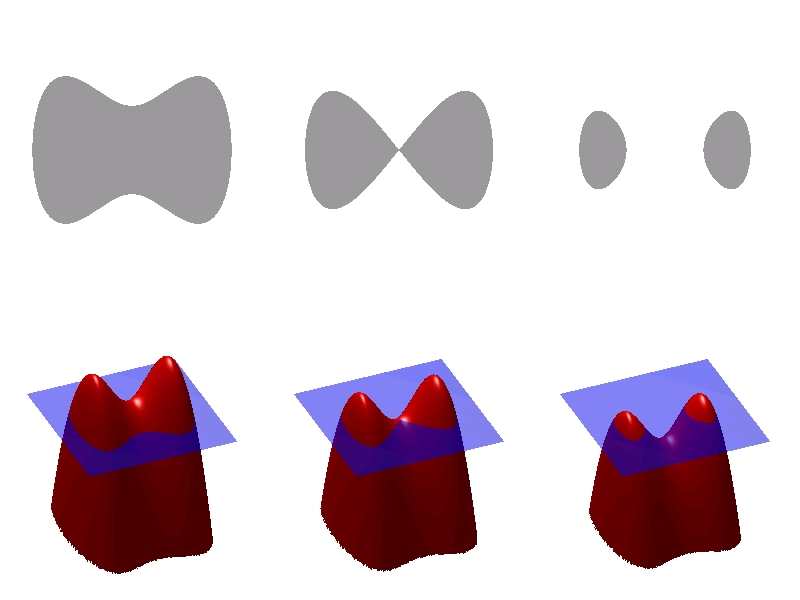
\includegraphics[width=0.9\textwidth]{../Art/Level_set_method.jpg}
\end{center}

\end{columns}

\end{frame}

%%%%%%%%%%%%%%%%%%%%%%%%%%%%%%%%%%%%%%%%%%%%%%%%%%%%%%%%%%%%%%%%%%%%%%%%%%%%%%%%
%%%%%%%%%%%%%%%%%%%%%%%%%%%%%%%%%%%%%%%%%%%%%%%%%%%%%%%%%%%%%%%%%%%%%%%%%%%%%%%%
%%%%%%%%%%%%%%%%%%%%%%%%%%%%%%%%%%%%%%%%%%%%%%%%%%%%%%%%%%%%%%%%%%%%%%%%%%%%%%%%

\begin{frame}
\frametitle{Level-Set Evolution}
\begin{itemize}
  \item Deforms the level-set function
  \begin{itemize}
    \item Driven by given PDE
    \begin{itemize}
      \item<2->[Regularized Advection]
      \begin{equation*}
      \frac{\partial \phi}{\partial \tau} = 
      \alpha \cdot \overrightarrow{A}(p) \bullet \overrightarrow{\nabla} \phi +
      \gamma \cdot \text{div}\left( \frac{\overrightarrow{\nabla}
      \phi}{\|\overrightarrow{\nabla} \phi\|} \right) \cdot
    \|\overrightarrow{\nabla}
      \phi\|
      \end{equation*}
      \only<2>{
      \begin{columns}
        \column{0.3\textwidth}
        \begin{block}{Advection}
        \begin{center}
          $\alpha \cdot \overrightarrow{A}(p) \bullet \overrightarrow{\nabla}
\phi$ \\
        \end{center}
        $\alpha$: coefficient\\
        $A(p)$: Advection field
        \end{block}

        \column{0.3\textwidth}
        \begin{block}{Curvature}
        \begin{center}
          $\gamma \cdot \|\overrightarrow{\nabla} \phi\| \cdot 
            \text{div}\ \frac{\overrightarrow{\nabla}
            \phi}{\|\overrightarrow{\nabla} \phi\|}$\\
        \end{center}
          $\gamma$: coefficient
        \end{block}
      \end{columns}
    }

      \item<3->[Regularized Propagation]
      \begin{equation*}
      \frac{\partial \phi}{\partial \tau} = 
      \beta \cdot P(p) \cdot \|\overrightarrow{\nabla} \phi \| +
      \gamma \cdot \text{div}\left( \frac{\overrightarrow{\nabla}
      \phi}{\|\overrightarrow{\nabla} \phi\|} \right) \cdot
    \|\overrightarrow{\nabla}
      \phi\|
      \end{equation*}
      \only<3>{
      \begin{columns}
        \column{0.3\textwidth}
        \begin{block}<3>{Propagation}
          \begin{center}
          $\beta \cdot P(p) \cdot \|\overrightarrow{\nabla} \phi\|$ \\
          \end{center}
          $\beta$: coefficient \\
          $P(p)$: Propagation field
        \end{block}

        \column{0.3\textwidth}
        \begin{block}{Curvature}
          \begin{center}
          $\gamma \cdot \|\overrightarrow{\nabla} \phi\| \cdot 
            \text{div}\ \frac{\overrightarrow{\nabla}
            \phi}{\|\overrightarrow{\nabla} \phi\|}$\\
          \end{center}
          $\gamma$: coefficient
        \end{block}
      \end{columns}
      }
      \item<4->[Chan and Vese]
      \begin{equation*}
      \frac{\partial \phi}{\partial \tau} = \delta_{\epsilon}(\phi) 
      \left(
      - \lambda_{in} \left( I - \mu_{in} \right) + 
      \lambda_{out} \left( I - \mu_{out} \right)
      \right)
      \end{equation*}
      \only<4>{
      \begin{columns}
        \column{0.3\textwidth}
        \begin{block}{Chan And Vese Internal}
          \begin{center}
          $\delta_{\epsilon}(\phi) \left( \lambda_{in} \left( I - \mu_{in}
\right)\right)$ \\
          \end{center}
          $\lambda_{in}$: coefficient \\
          $\mu_{in}$: Internal Mean
        \end{block}

        \column{0.3\textwidth}
        \begin{block}{Chan And Vese External}
          \begin{center}
          $\delta_{\epsilon}(\phi) \left( \lambda_{out} \left( I - \mu_{out}
\right)\right)$ \\
          \end{center}
          $\lambda_{out}$: coefficient \\
          $\mu_{out}$: External Mean
        \end{block}
      \end{columns}
      }
    \end{itemize}
  \end{itemize}
\end{itemize}
\end{frame}

%%%%%%%%%%%%%%%%%%%%%%%%%%%%%%%%%%%%%%%%%%%%%%%%%%%%%%%%%%%%%%%%%%%%%%%%%%%%%%%%
%%%%%%%%%%%%%%%%%%%%%%%%%%%%%%%%%%%%%%%%%%%%%%%%%%%%%%%%%%%%%%%%%%%%%%%%%%%%%%%%
%%%%%%%%%%%%%%%%%%%%%%%%%%%%%%%%%%%%%%%%%%%%%%%%%%%%%%%%%%%%%%%%%%%%%%%%%%%%%%%%

\begin{frame}
\frametitle{Level-Set Evolution}
\begin{itemize}
  \item Iterative computation
  \item Topological flexibility
\end{itemize}
\end{frame}


%%%%%%%%%%%%%%%%%%%%%%%%%%%%%%%%%%%%%%%%%%%%%%%%%%%%%%%%%%%%%%%%%%%%%%%%%%%%%%%%
%%%%%%%%%%%%%%%%%%%%%%%%%%%%%%%%%%%%%%%%%%%%%%%%%%%%%%%%%%%%%%%%%%%%%%%%%%%%%%%%
%%%%%%%%%%%%%%%%%%%%%%%%%%%%%%%%%%%%%%%%%%%%%%%%%%%%%%%%%%%%%%%%%%%%%%%%%%%%%%%%

\begin{frame}
\frametitle{Level Sets: Challenges in Segmentation?}
\begin{itemize}
  \item PDE Term choice
    \begin{itemize}
      \item Advection terms ?
      \item Propagation terms ?
      \item Region terms ?
      \item Regularization terms ?
    \end{itemize}
  \item<2-> Stopping criterion
    \begin{itemize}
      \item Number of Iterations ?
      \item Variation of interface length / area ?
      \item Variation of shape area / volume ?
    \end{itemize}
  \item<3-> PDE Parameters tuning
\end{itemize}
\end{frame}

%%%%%%%%%%%%%%%%%%%%%%%%%%%%%%%%%%%%%%%%%%%%%%%%%%%%%%%%%%%%%%%%%%%%%%%%%%%%%%%%
%%%%%%%%%%%%%%%%%%%%%%%%%%%%%%%%%%%%%%%%%%%%%%%%%%%%%%%%%%%%%%%%%%%%%%%%%%%%%%%%
%%%%%%%%%%%%%%%%%%%%%%%%%%%%%%%%%%%%%%%%%%%%%%%%%%%%%%%%%%%%%%%%%%%%%%%%%%%%%%%%



\section{Overview of the Level-Sets in ITKv4}
\centeredlargetext{white}{black}{
Overview of the Level-Sets in ITKv4
}

%%%%%%%%%%%%%%%%%%%%%%%%%%%%%%%%%%%%%%%%%%%%%%%%%%%%%%%%%%%%%%%%%%%%%%%%%%%%%%%%
%%%%%%%%%%%%%%%%%%%%%%%%%%%%%%%%%%%%%%%%%%%%%%%%%%%%%%%%%%%%%%%%%%%%%%%%%%%%%%%%
%%%%%%%%%%%%%%%%%%%%%%%%%%%%%%%%%%%%%%%%%%%%%%%%%%%%%%%%%%%%%%%%%%%%%%%%%%%%%%%%

\begin{frame}
\frametitle{Level Sets Representation}
\begin{columns}
\column{0.45\textwidth}
\begin{block}{Discrete}
  \begin{itemize}
  \item Dense
  \item<2-> Sparse
  \begin{enumerate}
      \item<3-> Whitaker  
      \item<4-> Shi       
      \item<5-> Malcolm   
    \end{enumerate}
  \end{itemize}
\end{block}

\begin{block}<6->{Parametric}
  \begin{itemize}
    \item \alert{Easy integration of new representation}
  \end{itemize}
\end{block}

\column{0.45\textwidth}
\only<3>{
\begin{center}
 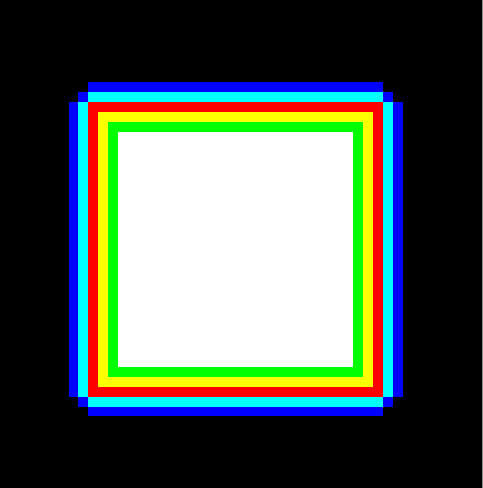
\includegraphics[width=0.8\textwidth]{../Art/WhitakerLayers.png}
 % WhitakerLayers.png: 483x488 pixel, 72dpi, 17.04x17.21 cm, bb=0 0 483 488
\end{center}
}
\only<4>{
\begin{center}
 
\includegraphics[width=0.8\textwidth]{../Art/ShiLayers.png}
 % WhitakerLayers.png: 483x488 pixel, 72dpi, 17.04x17.21 cm, bb=0 0 483 488
\end{center}
}
\only<5->{
\begin{center}
 
\includegraphics[width=0.8\textwidth]{../Art/MalcolmLayers.png}
 % WhitakerLayers.png: 483x488 pixel, 72dpi, 17.04x17.21 cm, bb=0 0 483 488
\end{center}
}

\end{columns}

\end{frame}

%%%%%%%%%%%%%%%%%%%%%%%%%%%%%%%%%%%%%%%%%%%%%%%%%%%%%%%%%%%%%%%%%%%%%%%%%%%%%%%%
%%%%%%%%%%%%%%%%%%%%%%%%%%%%%%%%%%%%%%%%%%%%%%%%%%%%%%%%%%%%%%%%%%%%%%%%%%%%%%%%
%%%%%%%%%%%%%%%%%%%%%%%%%%%%%%%%%%%%%%%%%%%%%%%%%%%%%%%%%%%%%%%%%%%%%%%%%%%%%%%%

\begin{frame}
\frametitle{Level Sets Equation}

\begin{columns}
  \column{0.47\textwidth} 
  \begin{block}{Term}
    \begin{itemize}
      \item Contribution for $\phi$ evolution
      \item Contribution for time step computation
      \item Coefficient
    \end{itemize} 
  \alert<2->{Easy to contribute new terms!}
  \end{block}

  \column{0.47\textwidth}
  \begin{block}<3->{TermContainer}
    \begin{itemize}
      \item Represent a given PDEs
      \item Mix of any term
      \item Independant of the representation
    \end{itemize}
  \alert<4->{Easy to contribute new PDEs!}
  \end{block}

\end{columns}

\end{frame}

%%%%%%%%%%%%%%%%%%%%%%%%%%%%%%%%%%%%%%%%%%%%%%%%%%%%%%%%%%%%%%%%%%%%%%%%%%%%%%%%
%%%%%%%%%%%%%%%%%%%%%%%%%%%%%%%%%%%%%%%%%%%%%%%%%%%%%%%%%%%%%%%%%%%%%%%%%%%%%%%%
%%%%%%%%%%%%%%%%%%%%%%%%%%%%%%%%%%%%%%%%%%%%%%%%%%%%%%%%%%%%%%%%%%%%%%%%%%%%%%%%

\begin{frame}
\frametitle{Other Features}
  \begin{itemize}
    \item N Level-Sets function evolving at the same time
    \item Geometrical Constraints
  \end{itemize}
\end{frame}

%%%%%%%%%%%%%%%%%%%%%%%%%%%%%%%%%%%%%%%%%%%%%%%%%%%%%%%%%%%%%%%%%%%%%%%%%%%%%%%%
%%%%%%%%%%%%%%%%%%%%%%%%%%%%%%%%%%%%%%%%%%%%%%%%%%%%%%%%%%%%%%%%%%%%%%%%%%%%%%%%
%%%%%%%%%%%%%%%%%%%%%%%%%%%%%%%%%%%%%%%%%%%%%%%%%%%%%%%%%%%%%%%%%%%%%%%%%%%%%%%%
\subsection{Example}

%%%%%%%%%%%%%%%%%%%%%%%%%%%%%%%%%%%%%%%%%%%%%%%%%%%%%%%%%%%%%%%%%%%%%%%%%%%%%%%%
%%%%%%%%%%%%%%%%%%%%%%%%%%%%%%%%%%%%%%%%%%%%%%%%%%%%%%%%%%%%%%%%%%%%%%%%%%%%%%%%
%%%%%%%%%%%%%%%%%%%%%%%%%%%%%%%%%%%%%%%%%%%%%%%%%%%%%%%%%%%%%%%%%%%%%%%%%%%%%%%%

\begin{frame}[fragile]
  \frametitle{How to run the example?}
  \fontsize{8pt}{8pt}\selectfont
\begin{verbatim}
cd ~/bin/ITKv4-TheNextGeneration-Tutorial/bin/
./SingleLevelSetWhitaker <InputImage> <NumberOfIterations> \
  <Visualization (0 or 1)> <OutputImage>
./SingleLevelSetWhitaker ~/src/ITKv4-TheNextGeneration-Tutortial/Exercises/LevelSets/Input/cells.png \
  800 1 cells_segmented.mha
\end{verbatim}
\end{frame}
\centeredlargetext{white}{black}{
Example
}

\begin{frame}
  \frametitle{Create a level-set function from binary mask}
  \lstlistingwithnumber{87}{94}{SingleLevelSetWhitaker.cxx}
  \lstlistingwithnumber{98}{100}{SingleLevelSetWhitaker.cxx}
\end{frame}

%%%%%%%%%%%%%%%%%%%%%%%%%%%%%%%%%%%%%%%%%%%%%%%%%%%%%%%%%%%%%%%%%%%%%%%%%%%%%%%%
%%%%%%%%%%%%%%%%%%%%%%%%%%%%%%%%%%%%%%%%%%%%%%%%%%%%%%%%%%%%%%%%%%%%%%%%%%%%%%%%
%%%%%%%%%%%%%%%%%%%%%%%%%%%%%%%%%%%%%%%%%%%%%%%%%%%%%%%%%%%%%%%%%%%%%%%%%%%%%%%%

\begin{frame}
  \frametitle{Create a domain for the level-set function}
  \lstlistingwithnumber{106}{110}{SingleLevelSetWhitaker.cxx}
  \lstlistingwithnumber{114}{125}{SingleLevelSetWhitaker.cxx}
\end{frame}

%%%%%%%%%%%%%%%%%%%%%%%%%%%%%%%%%%%%%%%%%%%%%%%%%%%%%%%%%%%%%%%%%%%%%%%%%%%%%%%%
%%%%%%%%%%%%%%%%%%%%%%%%%%%%%%%%%%%%%%%%%%%%%%%%%%%%%%%%%%%%%%%%%%%%%%%%%%%%%%%%
%%%%%%%%%%%%%%%%%%%%%%%%%%%%%%%%%%%%%%%%%%%%%%%%%%%%%%%%%%%%%%%%%%%%%%%%%%%%%%%%

\begin{frame}
  \frametitle{Setting up the level-set container}
  \lstlistingwithnumber{129}{135}{SingleLevelSetWhitaker.cxx}
  \lstlistingwithnumber{137}{144}{SingleLevelSetWhitaker.cxx}
\end{frame}

%%%%%%%%%%%%%%%%%%%%%%%%%%%%%%%%%%%%%%%%%%%%%%%%%%%%%%%%%%%%%%%%%%%%%%%%%%%%%%%%
%%%%%%%%%%%%%%%%%%%%%%%%%%%%%%%%%%%%%%%%%%%%%%%%%%%%%%%%%%%%%%%%%%%%%%%%%%%%%%%%
%%%%%%%%%%%%%%%%%%%%%%%%%%%%%%%%%%%%%%%%%%%%%%%%%%%%%%%%%%%%%%%%%%%%%%%%%%%%%%%%

\begin{frame}
  \frametitle{Setting up the level-set container}
  \lstlistingwithnumber{129}{135}{SingleLevelSetWhitaker.cxx}
  \lstlistingwithnumber{137}{144}{SingleLevelSetWhitaker.cxx}
\end{frame}

%%%%%%%%%%%%%%%%%%%%%%%%%%%%%%%%%%%%%%%%%%%%%%%%%%%%%%%%%%%%%%%%%%%%%%%%%%%%%%%%
%%%%%%%%%%%%%%%%%%%%%%%%%%%%%%%%%%%%%%%%%%%%%%%%%%%%%%%%%%%%%%%%%%%%%%%%%%%%%%%%
%%%%%%%%%%%%%%%%%%%%%%%%%%%%%%%%%%%%%%%%%%%%%%%%%%%%%%%%%%%%%%%%%%%%%%%%%%%%%%%%

\begin{frame}
  \frametitle{Creating PDE Terms}
  \begin{itemize}
    \item Chan and Vese internal term
    \lstlistingwithnumber{151}{158}{SingleLevelSetWhitaker.cxx}
    \item Chan and Vese external term
    \lstlistingwithnumber{162}{169}{SingleLevelSetWhitaker.cxx}
  \end{itemize}
\end{frame}

%%%%%%%%%%%%%%%%%%%%%%%%%%%%%%%%%%%%%%%%%%%%%%%%%%%%%%%%%%%%%%%%%%%%%%%%%%%%%%%%
%%%%%%%%%%%%%%%%%%%%%%%%%%%%%%%%%%%%%%%%%%%%%%%%%%%%%%%%%%%%%%%%%%%%%%%%%%%%%%%%
%%%%%%%%%%%%%%%%%%%%%%%%%%%%%%%%%%%%%%%%%%%%%%%%%%%%%%%%%%%%%%%%%%%%%%%%%%%%%%%%

\begin{frame}
  \frametitle{Setting up PDE}
  \lstlistingwithnumber{174}{178}{SingleLevelSetWhitaker.cxx}
  \lstlistingwithnumber{180}{181}{SingleLevelSetWhitaker.cxx}
  \lstlistingwithnumber{185}{188}{SingleLevelSetWhitaker.cxx}
\end{frame}

%%%%%%%%%%%%%%%%%%%%%%%%%%%%%%%%%%%%%%%%%%%%%%%%%%%%%%%%%%%%%%%%%%%%%%%%%%%%%%%%
%%%%%%%%%%%%%%%%%%%%%%%%%%%%%%%%%%%%%%%%%%%%%%%%%%%%%%%%%%%%%%%%%%%%%%%%%%%%%%%%
%%%%%%%%%%%%%%%%%%%%%%%%%%%%%%%%%%%%%%%%%%%%%%%%%%%%%%%%%%%%%%%%%%%%%%%%%%%%%%%%

\begin{frame}
  \frametitle{Stopping criterion}
  \lstlistingwithnumber{193}{196}{SingleLevelSetWhitaker.cxx}
\end{frame}

%%%%%%%%%%%%%%%%%%%%%%%%%%%%%%%%%%%%%%%%%%%%%%%%%%%%%%%%%%%%%%%%%%%%%%%%%%%%%%%%
%%%%%%%%%%%%%%%%%%%%%%%%%%%%%%%%%%%%%%%%%%%%%%%%%%%%%%%%%%%%%%%%%%%%%%%%%%%%%%%%
%%%%%%%%%%%%%%%%%%%%%%%%%%%%%%%%%%%%%%%%%%%%%%%%%%%%%%%%%%%%%%%%%%%%%%%%%%%%%%%%

\begin{frame}
  \frametitle{Starts the evolution}
  \begin{itemize}
    \item Set a stopping criterion
    \lstlistingwithnumber{193}{196}{SingleLevelSetWhitaker.cxx}
    \item Evolve
    \lstlistingwithnumber{198}{204}{SingleLevelSetWhitaker.cxx}
    \lstlistingwithnumber{208}{208}{SingleLevelSetWhitaker.cxx}
  \end{itemize}
\end{frame}

%%%%%%%%%%%%%%%%%%%%%%%%%%%%%%%%%%%%%%%%%%%%%%%%%%%%%%%%%%%%%%%%%%%%%%%%%%%%%%%%
%%%%%%%%%%%%%%%%%%%%%%%%%%%%%%%%%%%%%%%%%%%%%%%%%%%%%%%%%%%%%%%%%%%%%%%%%%%%%%%%
%%%%%%%%%%%%%%%%%%%%%%%%%%%%%%%%%%%%%%%%%%%%%%%%%%%%%%%%%%%%%%%%%%%%%%%%%%%%%%%%

\subsection{Exercise 1}
\centeredlargetext{white}{black}{
Exercise 1: Add a curvature term to LevelSetExercise1.cxx
}

%%%%%%%%%%%%%%%%%%%%%%%%%%%%%%%%%%%%%%%%%%%%%%%%%%%%%%%%%%%%%%%%%%%%%%%%%%%%%%%%
%%%%%%%%%%%%%%%%%%%%%%%%%%%%%%%%%%%%%%%%%%%%%%%%%%%%%%%%%%%%%%%%%%%%%%%%%%%%%%%%
%%%%%%%%%%%%%%%%%%%%%%%%%%%%%%%%%%%%%%%%%%%%%%%%%%%%%%%%%%%%%%%%%%%%%%%%%%%%%%%%

\subsection{Exercise 2}
\centeredlargetext{white}{black}{
Exercise 2: Change represesentation from Whitaker's to Shi's in
LevelSetExercise2.cxx
}

% \begin{frame}
% \frametitle{Multi Level Sets}
% \begin{itemize}
%   \item N Level Sets function evolving at the same time
%   \item Geometrical Constraints
% \end{itemize}
% \end{frame}
% 
% \end{colum}


% \section{Virtual Machines Preparation}

\centeredlargetext{white}{black}{
Virtual Machines Preparation
}

\begin{frame}
\frametitle{Virtual Machines Preparation}
\begin{itemize}
\item Get DVD / USB Memory Stick
\item Install VirtualBox from it
\item Import the VirtualMachine file
\item Boot the Virtual Machine
\item Log in
\item Get familiar with directories
\end{itemize}
\end{frame}


\begin{frame}
\frametitle{Media Content}
\framesubtitle{Directories and Files}
\begin{itemize}
\item VirtualBoxInstallers
\begin{itemize}
\item VirtualBox-4.0.8-71778-OSX.dmg (Mac)
\item VirtualBox-4.0.8-71778-Win.exe (Windows)
\item (Ubuntu Linux)
\begin{itemize}
\item virtualbox-4.0\_4.0.8-71778~Ubuntu~lucid\_amd64.deb
\item virtualbox-4.0\_4.0.8-71778~Ubuntu~lucid\_i386.deb
\item virtualbox-4.0\_4.0.8-71778~Ubuntu~maverick\_amd64.deb
\item virtualbox-4.0\_4.0.8-71778~Ubuntu~maverick\_i386.deb
\item virtualbox-4.0\_4.0.8-71778~Ubuntu~natty\_amd64.deb
\item virtualbox-4.0\_4.0.8-71778~Ubuntu~natty\_i386.deb
\item \ldots
\end{itemize}
\end{itemize}
\pause
\item VirtualMachine
\begin{itemize}
\item  OpenCV-ITK-disk1.vmdk
\item  OpenCV-ITK.ovf
\end{itemize}
\end{itemize}
\end{frame}

\begin{frame}
\frametitle{Install VirtualBox}
\begin{itemize}
\item Select the installer for your platform
\item Run it
\end{itemize}
\end{frame}

\begin{frame}
\frametitle{Alternative Linux Installation}
\begin{itemize}
\item  You can also install VirtualBox by doing:
\item  sudo apt-get install virtualbox-ose-qt
\end{itemize}
\end{frame}

\begin{frame}
\frametitle{Importing the Virtual Machine}
\begin{itemize}
\item Run VirtualBox
\item In ``File'' Menu select ``Import Appliance''
\item Provide the filename in the DVD / USB stick ``VirtualMachine/OpenCV-ITK.ovf"
\item A progress bar will appear, and when it finishes you should see:
\end{itemize}
\begin{center}
  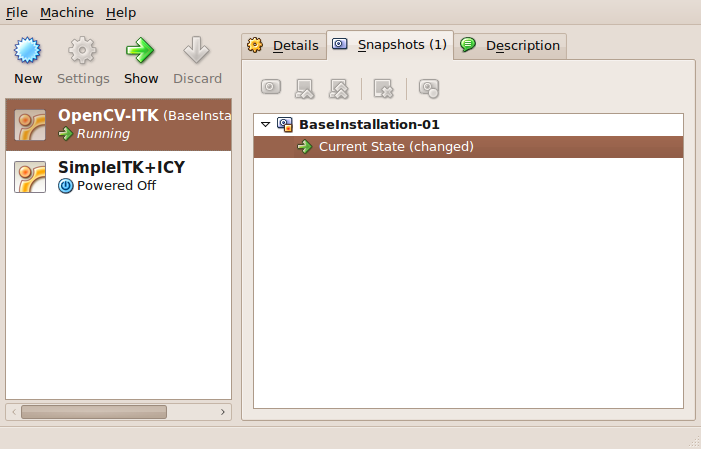
\includegraphics[width=0.5\paperwidth]{Screenshot-VirtualBox-OSE-01.png}
\end{center}
\end{frame}


\centeredlargetext{white}{black}{
We will get back...
}


% \include{ITKOverview}

% \section{Virtual Machines Preparation II}

\centeredlargetext{white}{black}{
Virtual Machine Preparation II
}

\subsection{Booting the Virtual Machine}
\begin{frame}
\frametitle{Booting the Virtual Machine}
\begin{itemize}
\item Click on the ``ITKv4'' icon on the left, to select it.
\item Click on the Green Arrow at the top ``Show''.
\item The VM will start to boot and you will see the warning:
\end{itemize}
\begin{center}
  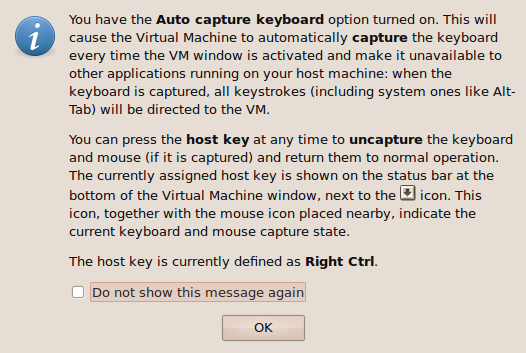
\includegraphics[width=0.4\paperwidth]{../Art/Screenshot-VirtualBox-OSE-02.png}
\end{center}
\begin{itemize}
\item Click ``OK''
\end{itemize}
\end{frame}

\begin{frame}
\frametitle{Booting the Virtual Machine}
\begin{itemize}
\item The boot sequence should continue and you should see:
\end{itemize}
\begin{center}
  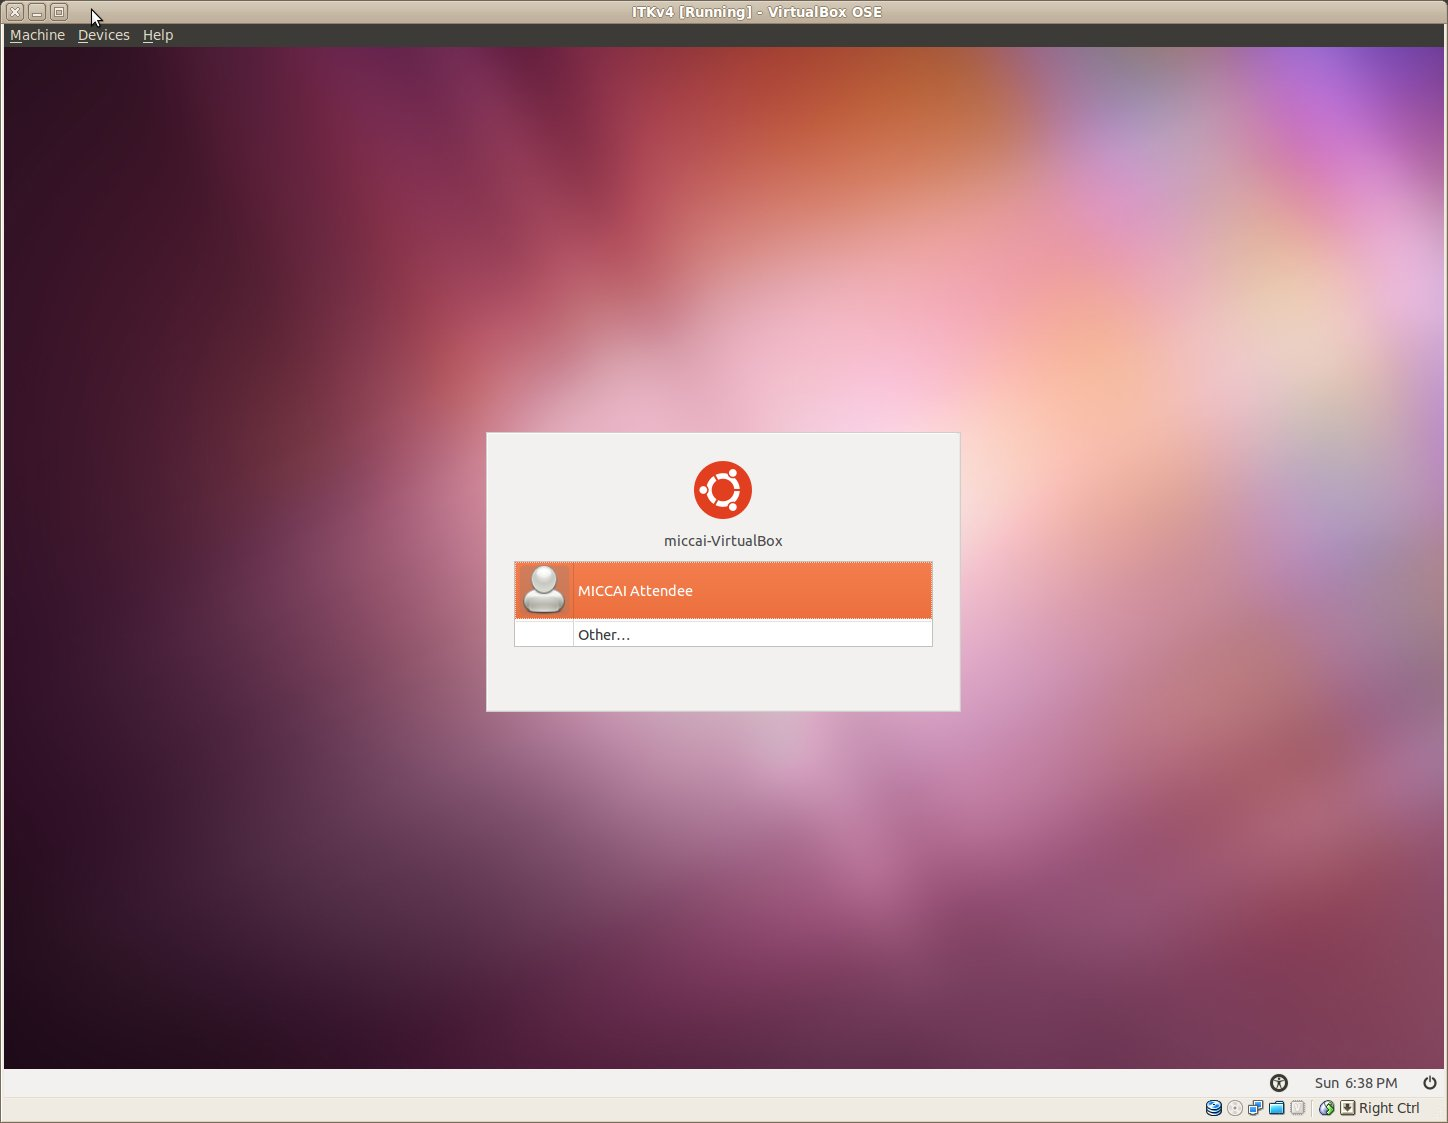
\includegraphics[width=0.7\paperwidth]{../Art/Screenshot-ITKv4-VirtualBox-01.jpg}
\end{center}
\begin{itemize}
\item Login with the password: ``toronto''
\end{itemize}
\end{frame}

\begin{frame}
\frametitle{Booting the Virtual Machine}
\begin{itemize}
\item After logging in you should see:
\end{itemize}
\begin{center}
  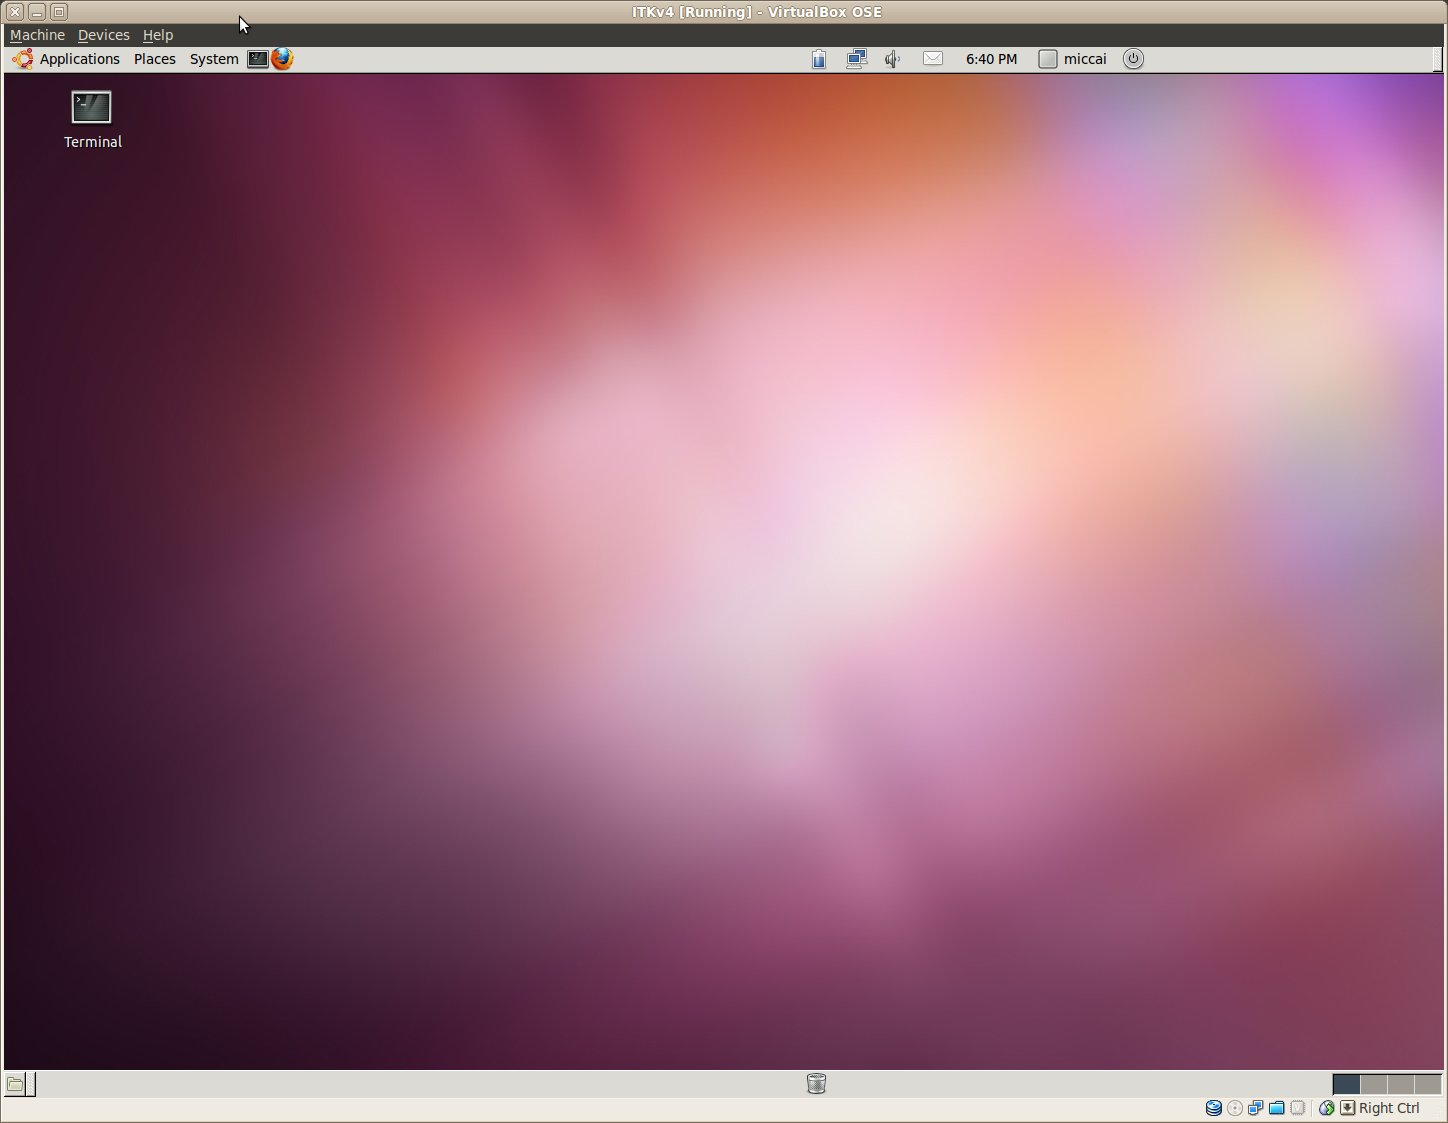
\includegraphics[width=0.7\paperwidth]{../Art/Screenshot-ITKv4-VirtualBox-02.jpg}
\end{center}
\end{frame}


\centeredlargetext{white}{black}{
Your Virtual Machine\\ is Ready !
}

\begin{frame}
\frametitle{Additional Copies}
\begin{itemize}
\item The same source trees are available in the DVD / USB key
\item Outside of the VirtualBox image
\end{itemize}
\end{frame}



% \subsection{Software Environment}

\centeredlargetext{white}{black}{
Software Environment
}

{
\setbeamertemplate{background}{}
\begin{frame}
\frametitle{Welcome to Debian GNU/Linux}
\begin{center}

\includegraphics[height=0.5\paperheight]{../Art/Tux.png}
%
\includegraphics[width=0.5\paperwidth]{../Art/blackeubuntulogo.png}
\end{center}
\end{frame}
}

{
\setbeamertemplate{background}{}
\begin{frame}
\frametitle{How to take the mouse out of the Virtual Machine}
\begin{itemize}
\item Hit the \textbf{RIGHT CTRL} Key on Windows / Linux Host
\item Hit the \textbf{LEFT APPLE} Key on Mac Host
\end{itemize}
\end{frame}
}

{
\setbeamertemplate{background}{}
\begin{frame}
\frametitle{How to Open a Terminal - Menu in Lower Left Corner}
\framesubtitle{To type your command line instructions}
\begin{center}
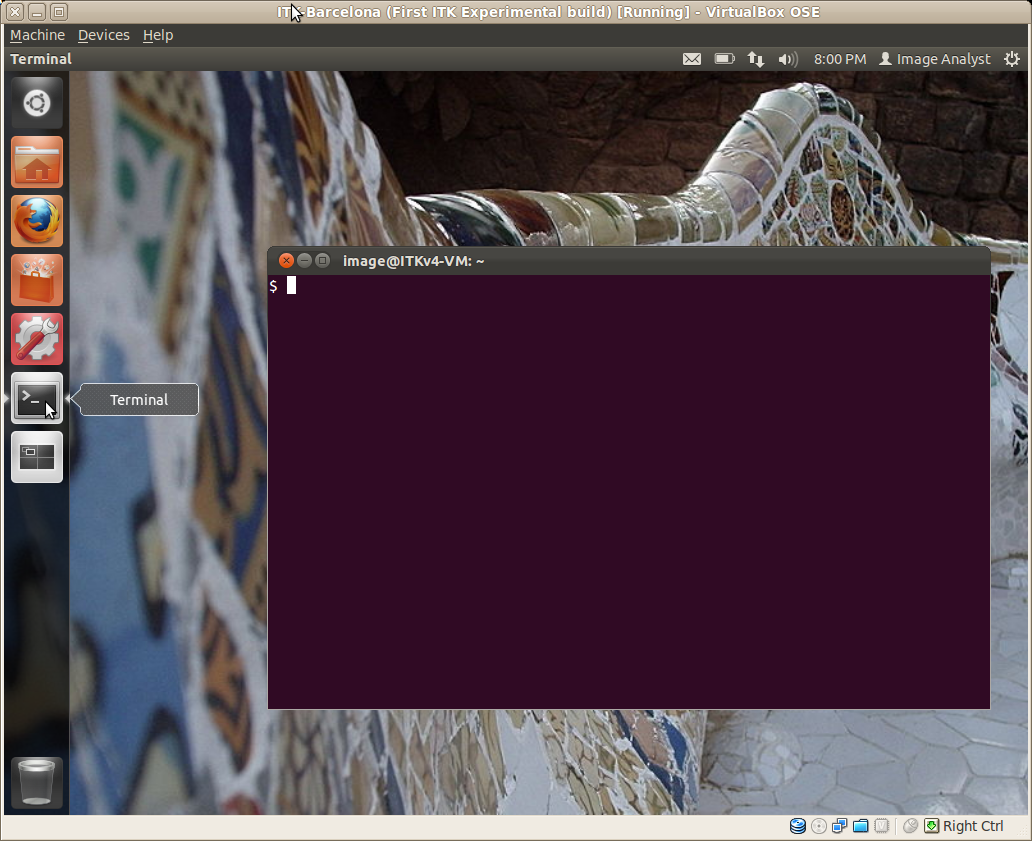
\includegraphics[width=0.7\paperwidth]{../Art/Screenshot-OpenTerminal.jpg}
\end{center}
\end{frame}
}

{
\setbeamertemplate{background}{}
\begin{frame}
\frametitle{How to Navigate Directories}
\framesubtitle{Double Click in Folder Icons in the Desktop}
\begin{center}
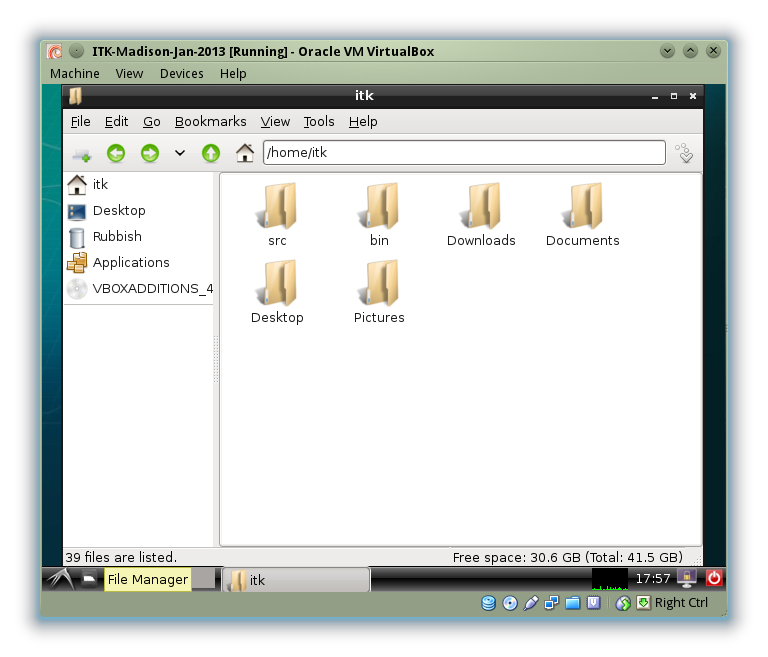
\includegraphics[width=0.7\paperwidth]{../Art/Screenshot-PCManFM.png}
\end{center}
\end{frame}
}

{
\setbeamertemplate{background}{}
\begin{frame}[fragile]
\frametitle{Walk through the directories}
\begin{itemize}
\item Find source code of exercises
\begin{verbatim}
cd ~/src/ITKv4-TheNextGeneration-Tutorial/Exercises
pwd
ls
pcmanfm .
\end{verbatim}
\pause
\item Find binary build of exercises
\begin{verbatim}
cd ~/bin/ITKv4-TheNextGeneration-Tutorial/Exercises
pwd
ls
\end{verbatim}
\end{itemize}
\end{frame}
}

{
\setbeamertemplate{background}{}
\begin{frame}[fragile]
\frametitle{The TAB Key is your Friend}
\begin{itemize}
\item When writing filenames
\item Use the TAB key for completions
\item No need to type full filenames
\end{itemize}
\end{frame}
}

{
\setbeamertemplate{background}{}
\begin{frame}[fragile]
\frametitle{How to View Images}
\begin{itemize}
\item Go to the directory
\item Invoke ``ImageViewer'' application
\begin{verbatim}
cd ~/data
ImageViewer BrainProtonDensitySlice.png
\end{verbatim}
\pause
\item Hit ``+'' key to zoom in
\pause
\item Hit ``-'' key to zoom out
\pause
\item Hit ESC key to quit the application
\end{itemize}
\end{frame}
}


% \include{ITKIntroduction}

% \section{OpenCV Introduction}


\centeredlargetext{white}{black}{
OpenCV Introduction
}


\begin{frame}
\frametitle{OpenCV Overview}
\begin{center}
\begin{columns}[c]
\column{0.8\textwidth}
\begin{itemize}
\item What is OpenCV?  OpenCV is \ldots
  \begin{itemize}
  \item an open source computer vision library.
  \item written in C, but has C++ and Python APIs.
  \item released under a BSD license.
  \item supported and guided by Willow Garage.
  \item found at \url{http://opencv.willowgarage.com/wiki/}.
  \end{itemize}
\end{itemize}
\column{0.2\textwidth}
 
\includegraphics[width=0.8\textwidth]{OpenCVLogo.png}
\end{columns}
\pause
\begin{itemize}
\item We will be using OpenCV 2.2 (from subversion).
\item The new C++ interface will be used when possible.
\item We assume you have some prior experience with OpenCV
\item \ldots but we will cover the basics in case you don't.
\end{itemize}
\end{center}
\end{frame}


\begin{frame}
\frametitle{Include Header Files}
\framesubtitle{OpenCVIntroduction/exercise1/BasicFilteringOpenCV.cxx}
\begin{center}
We need to include the OpenCV headers
\lstlistingwithnumber{19}{20}{BasicFilteringOpenCV.cxx}
\pause
\vspace{1 em}
and standard library headers for {\tt cout} and {\tt string}
\lstlistingwithnumber{22}{23}{BasicFilteringOpenCV.cxx}
\end{center}
\end{frame}


\begin{frame}
\frametitle{The Main function}
\framesubtitle{OpenCVIntroduction/exercise1/BasicFilteringOpenCV.cxx}
\begin{center}
\begin{itemize}
\lstlistingwithnumber{26}{52}{BasicFilteringOpenCV.cxx}
\end{itemize}
\end{center}
\end{frame}


\begin{frame}
\frametitle{Loading an Image / Applying a Filter}
\framesubtitle{OpenCVIntroduction/exercise1/BasicFilteringOpenCV.cxx}
\begin{center}
\begin{itemize}
\item If no arguments, print usage and exit \\
Note: {\tt argv[0]} contains the executable name
\lstlistingwithnumber{28}{32}{BasicFilteringOpenCV.cxx}
\pause
\item Load an image from the specified file into a matrix object
\lstlistingwithnumber{34}{34}{BasicFilteringOpenCV.cxx}
\pause
\item Create a matrix for the output and apply a median filter
\lstlistingwithnumber{35}{36}{BasicFilteringOpenCV.cxx}
\item The last argument represent the size of the filter, $9\times9$ in this case
\end{itemize}
\end{center}
\end{frame}


\begin{frame}
\frametitle{Displaying an Image}
\framesubtitle{OpenCVIntroduction/exercise1/BasicFilteringOpenCV.cxx}
\begin{center}
\begin{itemize}
\item If no output file is specified, use HighGUI to display the resulting image.
\lstlistingwithnumber{38}{45}{BasicFilteringOpenCV.cxx}
\end{itemize}
\end{center}
\end{frame}


\begin{frame}
\frametitle{Create the Display Window}
\framesubtitle{OpenCVIntroduction/exercise1/BasicFilteringOpenCV.cxx}
\begin{center}
\begin{itemize}
\item A title string is used to identify the GUI window.
\lstlistingwithnumber{40}{40}{BasicFilteringOpenCV.cxx}
\pause
\item Create a named window.
  \begin{itemize}
  \item {\tt\small CV\_WINDOW\_FREERATIO} is needed for display using OpenGL.
  \end{itemize}
\lstlistingwithnumber{41}{41}{BasicFilteringOpenCV.cxx}
\pause
\item Resize the window to match the image size.
  \begin{itemize}
  \item {\tt\small cvResizeWindow()} is a C function with no C++ API equivalent.
  \item It is not in the {\tt\small cv} namespace.
  \item It requires a {\tt\small const char*} name, provided by {\tt\small std::string::c\_str()}.
  \item The +50 in height to account for the height of tool/status bars.
  \end{itemize}
\lstlistingwithnumber{42}{42}{BasicFilteringOpenCV.cxx}
\end{itemize}
\end{center}
\end{frame}


\begin{frame}
\frametitle{Display and Wait}
\framesubtitle{OpenCVIntroduction/exercise1/BasicFilteringOpenCV.cxx}
\begin{center}
\begin{itemize}
\item Show the image in the previously created window.
\lstlistingwithnumber{43}{43}{BasicFilteringOpenCV.cxx}
\pause
\item Wait for the user to press a key, then continue.
\lstlistingwithnumber{44}{44}{BasicFilteringOpenCV.cxx}
\end{itemize}
\end{center}
\end{frame}


\begin{frame}
\frametitle{Saving an Image}
\framesubtitle{OpenCVIntroduction/exercise1/BasicFilteringOpenCV.cxx}
\begin{center}
\begin{itemize}
\item If an output file is specified, write the image to the specified file
\lstlistingwithnumber{46}{49}{BasicFilteringOpenCV.cxx}
\end{itemize}
\end{center}
\end{frame}


\begin{frame}[fragile]
\frametitle{Exercise 1}
\framesubtitle{OpenCVIntroduction/exercise1/BasicFilteringOpenCV.cxx}
\begin{center}
\begin{itemize}
\item Replace the median filter with a Canny edge detector
\lstlistingwithnumber{35}{36}{BasicFilteringOpenCV.cxx}
\pause
\item Hint: The OpenCV Canny function has this signature
\begin{lstlisting}[numbers=none,xleftmargin=0pt]
void Canny(const Mat& image, Mat& edges, double threshold1, double threshold2);
\end{lstlisting}
\pause
\item Canny requires grayscale image input, but our images are color
\item Hint: Use this function to convert a color space
\begin{lstlisting}[numbers=none,xleftmargin=0pt]
void cvtColor(const Mat& src, Mat& dst, int code);
\end{lstlisting}
\item Use {\tt CV\_BGR2GRAY} for {\tt code} to convert BGR color to gray.
\end{itemize}
\end{center}
\end{frame}


\begin{frame}[fragile]
\frametitle{Exercise 1: Answer}
\framesubtitle{OpenCVIntroduction/exercise1/BasicFilteringOpenCVAnswer.cxx}
\begin{center}
\lstlistingwithnumber{34}{38}{BasicFilteringOpenCVAnswer.cxx}
\begin{itemize}
\item Run \verb|./BasicFilteringOpenCV ~/data/mandrill.png|
\end{itemize}
\pause
\begin{columns}[c]
\column{0.5\textwidth}
\begin{center}
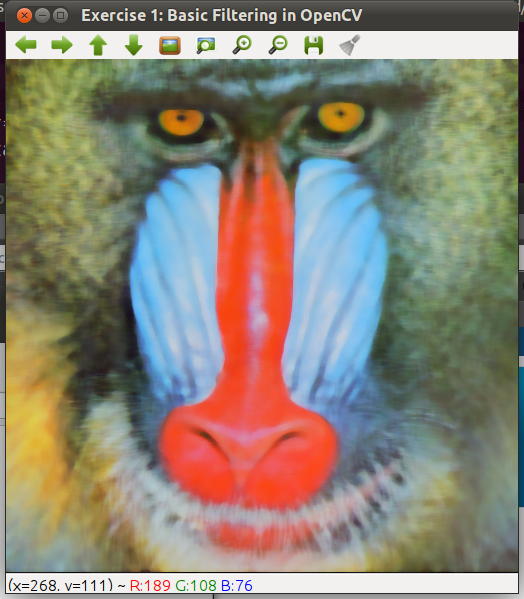
\includegraphics[width=0.5\textwidth]{OpenCVex1-GUI.png} \\
Median Filter
\end{center}
\column{0.5\textwidth}
\begin{center}
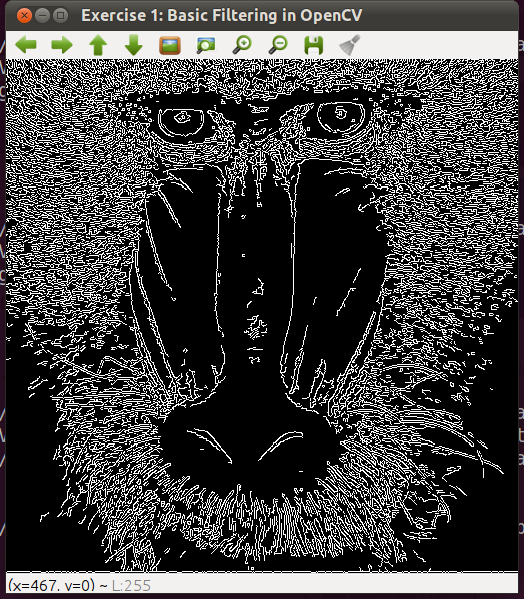
\includegraphics[width=0.5\textwidth]{OpenCVex1-ans-GUI.png} \\
Canny Edges
\end{center}
\end{columns}
\end{center}
\end{frame}


\begin{frame}
\frametitle{Exercise 2: Basic Video Filtering}
\framesubtitle{OpenCVIntroduction/exercise2/BasicVideoFilteringOpenCV.cxx}
\begin{center}
\begin{itemize}
\item Video filtering is similar to image filtering, except
  \begin{itemize}
  \item use a {\tt VideoCapture} object to read a video file.
  \item loop over each frame in the video and process each one.
  \item display or encode each output frame within the loop.
  \end{itemize}
\end{itemize}
\end{center}
\end{frame}


\begin{frame}
\frametitle{Loading a Video File}
\framesubtitle{OpenCVIntroduction/exercise2/BasicVideoFilteringOpenCV.cxx}
\begin{center}
\begin{itemize}
\item The first step is to open the video file and parse the headers.
\lstlistingwithnumber{88}{93}{BasicVideoFilteringOpenCV.cxx}
\item If unable to parse the headers then terminate the program.
\end{itemize}
\end{center}
\end{frame}


\begin{frame}
\frametitle{Display or Save}
\framesubtitle{OpenCVIntroduction/exercise2/BasicVideoFilteringOpenCV.cxx}
\begin{center}
\begin{itemize}
\item Same command line usage as before for selecting between displaying
      or saving results.
\item The processing code has been encapsulated into functions.
\item If only input video is specified, then display the resulting video.
\lstlistingwithnumber{95}{98}{BasicVideoFilteringOpenCV.cxx}
\item If a second file is specified, then save the resulting video to the file.
\lstlistingwithnumber{99}{102}{BasicVideoFilteringOpenCV.cxx}
\end{itemize}
\end{center}
\end{frame}


\begin{frame}
\frametitle{Prepare the Display Window}
\framesubtitle{OpenCVIntroduction/exercise2/BasicVideoFilteringOpenCV.cxx}
\begin{center}
\begin{itemize}
\item This function processes the video and displays the results.
\lstlistingwithnumber{35}{36}{BasicVideoFilteringOpenCV.cxx}
\pause
\item Use the {\tt\small get()} member function to access video properties: \\
      frame rate, width, and height.
\lstlistingwithnumber{37}{39}{BasicVideoFilteringOpenCV.cxx}
\pause
\item Setup the HighGUI window as in the previous example.
\lstlistingwithnumber{41}{43}{BasicVideoFilteringOpenCV.cxx}
\end{itemize}
\end{center}
\end{frame}


\begin{frame}
\frametitle{Process and Display}
\framesubtitle{OpenCVIntroduction/exercise2/BasicVideoFilteringOpenCV.cxx}
\begin{center}
\begin{itemize}
\item Number of milliseconds to wait before drawing the next frame.
\lstlistingwithnumber{45}{45}{BasicVideoFilteringOpenCV.cxx}
\pause
\item Loop until no more frames can be read from the video capture object.
\lstlistingwithnumber{47}{57}{BasicVideoFilteringOpenCV.cxx}
\item Call {\tt\small processFrame()} on each frame and and display the result.
\item {\tt waitkey(\emph{delay})} returns positive value indicating the key pressed
      or returns -1 after {\tt \emph{delay}} ms have passed.
\end{itemize}
\end{center}
\end{frame}


\begin{frame}
\frametitle{Create a Video Writer}
\framesubtitle{OpenCVIntroduction/exercise2/BasicVideoFilteringOpenCV.cxx}
\begin{center}
\begin{itemize}
\item This function processes the video and saves the results.
\lstlistingwithnumber{62}{63}{BasicVideoFilteringOpenCV.cxx}
\pause
\item Get the video properties as before.
\lstlistingwithnumber{64}{66}{BasicVideoFilteringOpenCV.cxx}
\pause
\item Specify that the output video will be encoded in DIVX format.
\item Create a video writer object with the specified filename.
\lstlistingwithnumber{68}{70}{BasicVideoFilteringOpenCV.cxx}
\end{itemize}
\end{center}
\end{frame}


\begin{frame}
\frametitle{Process and Save}
\framesubtitle{OpenCVIntroduction/exercise2/BasicVideoFilteringOpenCV.cxx}
\begin{center}
\begin{itemize}
\item Loop until no more frames can be read from the video capture object.
\lstlistingwithnumber{71}{76}{BasicVideoFilteringOpenCV.cxx}
\item Call {\tt\small processFrame()} on each frame.
\item Write the resulting image to the output video file with the insertion operator ({\tt\small <<}).
\end{itemize}
\end{center}
\end{frame}


\begin{frame}
\frametitle{Exercise 2}
\framesubtitle{OpenCVIntroduction/exercise2/BasicVideoFilteringOpenCV.cxx}
\begin{center}
\begin{itemize}
\item Implement {\tt\small processFrame()} by adding the Canny edge detector.
\lstlistingwithnumber{27}{31}{BasicVideoFilteringOpenCV.cxx}
\pause
\item Saving to a video requires color images, but Canny produces grayscale images.
\item Hint: Use {\tt\small cvtColor()} again to convert back to color.
\item Use code {\tt\small CV\_GRAY2BGR} for {\tt\small code} to convert gray to BGR.
\end{itemize}
\end{center}
\end{frame}


\begin{frame}[fragile]
\frametitle{Exercise 2: Answer}
\framesubtitle{OpenCVIntroduction/exercise2/BasicVideoFilteringOpenCVAnswer.cxx}
\begin{center}
\lstlistingwithnumber{27}{35}{BasicVideoFilteringOpenCVAnswer.cxx}
\begin{itemize}
\item Run \verb|./BasicVideoFilteringOpenCV ~/data/Walk1.mpg|
\end{itemize}
\pause
\begin{columns}[c]
\column{0.5\textwidth}
\begin{center}
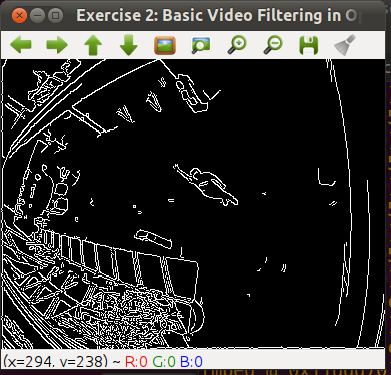
\includegraphics[width=0.5\textwidth]{OpenCVex2-ans-GUI.png} \\
HighGUI Display
\end{center}
\column{0.5\textwidth}
\begin{center}
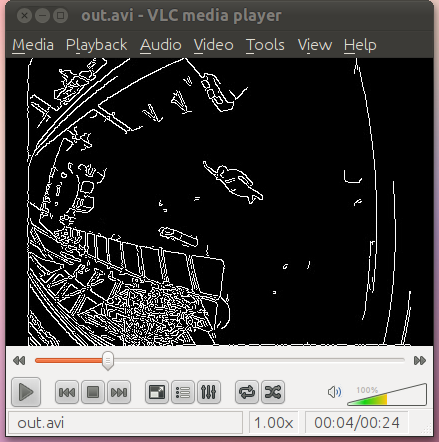
\includegraphics[width=0.5\textwidth]{OpenCVex2-ans-save.png} \\
Saved Video (Opened in vlc)
\end{center}
\end{columns}
\end{center}
\end{frame}


% \section{ITK OpenCV Bridge}

\subsection{OpenCV Introduction}

\centeredlargetext{white}{black}{
ITK OpenCV Bridge
}




\begin{frame}
\frametitle{OpenCV Overview}
\begin{center}
\begin{columns}[c]
\column{0.8\textwidth}
\begin{itemize}
\item What is OpenCV?  OpenCV is \ldots
  \begin{itemize}
  \item an open source computer vision library.
  \item written in C, but has C++ and Python APIs.
  \item released under a BSD license.
  \item supported and guided by Willow Garage.
  \item found at \url{http://opencv.willowgarage.com/wiki/}.
  \end{itemize}
\end{itemize}
\column{0.2\textwidth}
 
\includegraphics[width=0.8\textwidth]{../Art/OpenCVLogo.png}
\end{columns}
\pause
\begin{itemize}
\item We will be using OpenCV 2.4 (from subversion).
\end{itemize}
\end{center}
\end{frame}



\begin{frame}
\frametitle{Introduction}
\begin{itemize}
\item ITK Module for working with other libraries
\item Moving frame and/or video data between OpenCV and ITK
\item Bring biomedical and computer vision folks together
\end{itemize}
\end{frame}



\begin{frame}
\frametitle{Design Choices}
\begin{itemize}
\item OpenCV users and ITK users should both be comfortable
\item Image to image utility functions
\item cv::Source to itk::VideoStream
\item Video Group Modules: BridgeOpenCV,BridgeVXL,Core,Filterig,IO
\end{itemize}
\end{frame}

%-------------------------------------------
\subsection{Image Filtering}

\centeredlargetext{white}{black}{
Basic Image Filtering 
itk::image \& cv:mat}

\begin{frame}
\frametitle{Include Header Files}
\framesubtitle{ITKOpenCVBridge/exercise1/BasicFilteringITKOpenCVBridge.cxx}
\begin{itemize}
\item We include ITK and OpenCV headers (like before):
\lstlistingwithnumber{20}{21}{BasicFilteringITKOpenCVBridge.cxx}
\lstlistingwithnumber{23}{24}{BasicFilteringITKOpenCVBridge.cxx}
\item We also need to include the bridge header:
\lstlistingwithnumber{25}{25}{BasicFilteringITKOpenCVBridge.cxx}
\end{itemize}
\end{frame}

\begin{frame}
\frametitle{Basic Layout}
\framesubtitle{ITKOpenCVBridge/exercise1/BasicFilteringITKOpenCVBridge.cxx}
\begin{itemize}
\item The basic layout of this file is the same as the OpenCV
  Examples:
\lstlistingwithnumber{27}{35}{BasicFilteringITKOpenCVBridge.cxx}
\lstlistingwithnumber{69}{84}{BasicFilteringITKOpenCVBridge.cxx}
\end{itemize}
\end{frame}

\begin{frame}
\frametitle{Adding ITK}
\framesubtitle{ITKOpenCVBridge/exercise1/BasicFilteringITKOpenCVBridge.cxx}
\begin{itemize}
\item The type definitions should also be familiar from the ITK
  Material:
\lstlistingwithnumber{38}{45}{BasicFilteringITKOpenCVBridge.cxx}
\item However, notice the bridge class. It contains the conversion function
between OpenCV and ITK.
\lstlistingwithnumber{42}{42}{BasicFilteringITKOpenCVBridge.cxx}
\end{itemize}
\end{frame}

\begin{frame}
\frametitle{From OpenCV to ITK}
\framesubtitle{ITKOpenCVBridge/exercise1/BasicFilteringITKOpenCVBridge.cxx}
\begin{itemize}
\item We call our conversion function to go from a cv::Mat to an
  itk::Image
\lstlistingwithnumber{47}{48}{BasicFilteringITKOpenCVBridge.cxx}
\end{itemize}
\end{frame}

\begin{frame}
\frametitle{Filtering with ITK}
\framesubtitle{ITKOpenCVBridge/exercise1/BasicFilteringITKOpenCVBridge.cxx}
\begin{itemize}
\item The median filtering is normal ITK code, but we do not connect our
output to a writer
\lstlistingwithnumber{49}{64}{BasicFilteringITKOpenCVBridge.cxx}
\pause
\item Instead, we set it to our conversion function
\lstlistingwithnumber{66}{67}{BasicFilteringITKOpenCVBridge.cxx}
\end{itemize}
\end{frame}

\begin{frame}[fragile]
\frametitle{Running the Example}
\framesubtitle{ITKOpenCVBridge/exercise1/BasicFilteringITKOpenCVBridge.cxx}
\begin{itemize}
\item Run the example with the following command
\begin{verbatim}
      ./BasicFilteringITKOpenCVBridge     \
      ~/data/mandrillgray.png             \
      ./mandrillgrayMedian.png            

       eog .mandrillgrayMedian.png
\end{verbatim}
\end{itemize}
\end{frame}

\begin{frame}
\frametitle{Viewing the Results}
\framesubtitle{ITKOpenCVBridge/exercise1/BasicFilteringITKOpenCVBridge.cxx}
\begin{itemize}
\item Running the example the same way as before, we see a nicely
median-filtered image.
\end{itemize}
\begin{columns}[c]
\column{0.33\textwidth}
\begin{center}
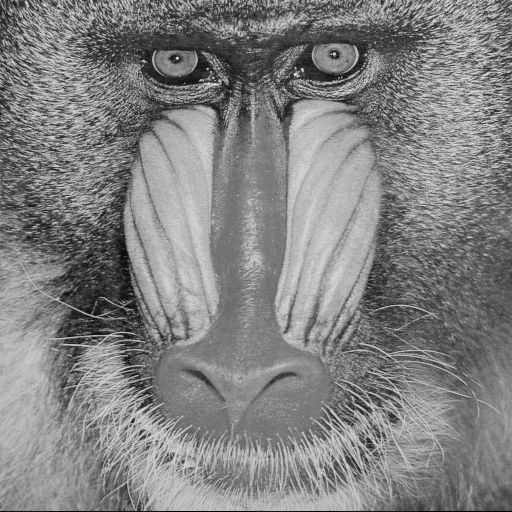
\includegraphics[width=1\textwidth]{../Art/mandrilgray.png} \\
Original
\end{center}
\column{0.33\textwidth}
\begin{center}
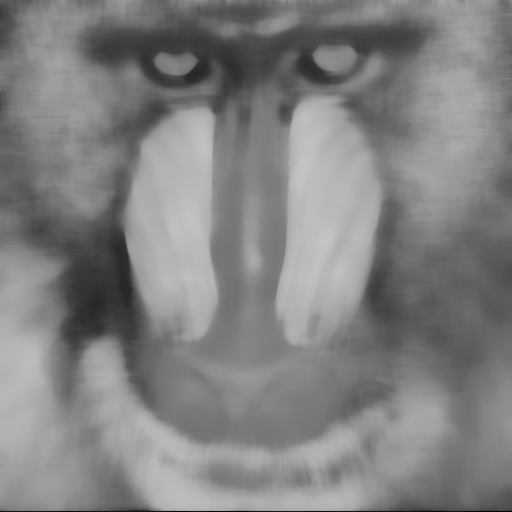
\includegraphics[width=1\textwidth]{../Art/OpenCVITKex1.png} \\
Median Filter
\end{center}
\end{columns}
\pause
\begin{itemize}
\item Now, the fun part. Let's modify our example to use Curvature Flow, an
anisotropic diffusion filter built into ITK.
\end{itemize}
\end{frame}


\begin{frame}
\begin{itemize}
\frametitle{Exercise 1}
\framesubtitle{ITKOpenCVBridge/exercise1/BasicFilteringITKOpenCVBridge.cxx}
\item Hint 1: Curvature Flow requires {\tt float} as the output pixel
  type.
\pause
\item Hint 2: Curvature Flow does not take a radius parameter. It's
  salient functions are:
\lstlistingwithnumber{50}{51}{BasicFilteringITKOpenCVBridgeAnswer.cxx}
\end{itemize}
\end{frame}

\begin{frame}
\begin{itemize}
\frametitle{Exercise 1: Answer}
\framesubtitle{ITKOpenCVBridge/exercise1/BasicFilteringITKOpenCVBridgeAnswer.cxx}
\item First, change the included filter
\lstlistingwithnumber{24}{24}{BasicFilteringITKOpenCVBridgeAnswer.cxx}
\pause
\item The type definitions also need to change to reflect the new
  filter and output image types.
\lstlistingwithnumber{37}{44}{BasicFilteringITKOpenCVBridgeAnswer.cxx}
\end{itemize}
\end{frame}

\begin{frame}
\begin{itemize}
\frametitle{Exercise 1: Answer}
\framesubtitle{ITKOpenCVBridge/exercise1/BasicFilteringITKOpenCVBridgeAnswer.cxx}
\item The semantics of calling the filter also has to change:
\lstlistingwithnumber{50}{51}{BasicFilteringITKOpenCVBridgeAnswer.cxx}
\pause
\item That's it! Now you're using a ``better'' blurring scheme.
\end{itemize}
\end{frame}

\begin{frame}
\begin{itemize}
\frametitle{Exercise 1: Answer}
\framesubtitle{ITKOpenCVBridge/exercise1/BasicFilteringITKOpenCVBridgeAnswer.cxx}
\item The final pipeline should look like this:
\lstlistingwithnumber{35}{35}{BasicFilteringITKOpenCVBridgeAnswer.cxx}
\lstlistingwithnumber{46}{62}{BasicFilteringITKOpenCVBridgeAnswer.cxx}
\end{itemize}
\end{frame}

\begin{frame}[fragile]
\frametitle{Running the Answer}
\framesubtitle{ITKOpenCVBridge/exercise1/BasicFilteringITKOpenCVBridgeAnswer.cxx}
\begin{itemize}
\item Run the answer with the following command
\begin{verbatim}
      ./BasicFilteringITKOpenCVBridgeAnswer     \
      ~/data/mandrillgray.png                   \
      ./mandrillgrayCurvatureFlow.png 
\end{verbatim}
\end{itemize}
\end{frame}

\begin{frame}
\begin{itemize}
\frametitle{Exercise 1: Answer}
\framesubtitle{ITKOpenCVBridge/exercise1/BasicFilteringITKOpenCVBridgeAnswer.cxx}
\item The results should look like this:
\end{itemize}
\begin{columns}[c]
\column{0.33\textwidth}
\begin{center}
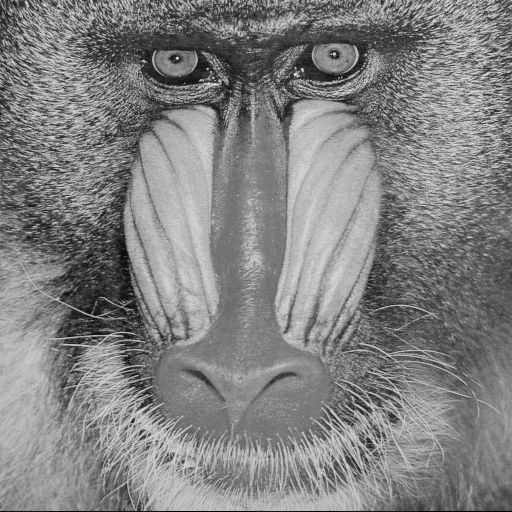
\includegraphics[width=1\textwidth]{../Art/mandrilgray.png} \\
Original
\end{center}
\column{0.33\textwidth}
\begin{center}
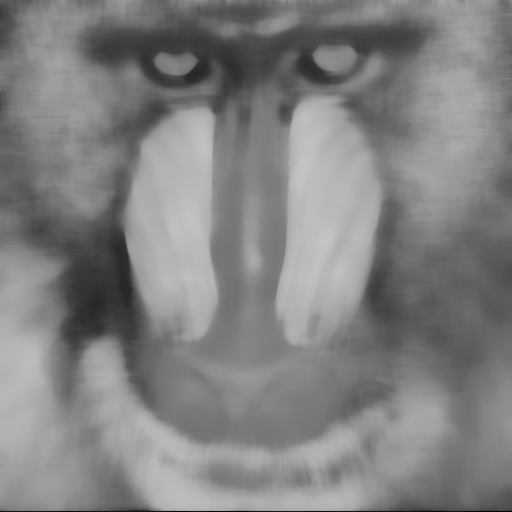
\includegraphics[width=1\textwidth]{../Art/OpenCVITKex1.png} \\
Median Filter
\end{center}
\column{0.33\textwidth}
\begin{center}
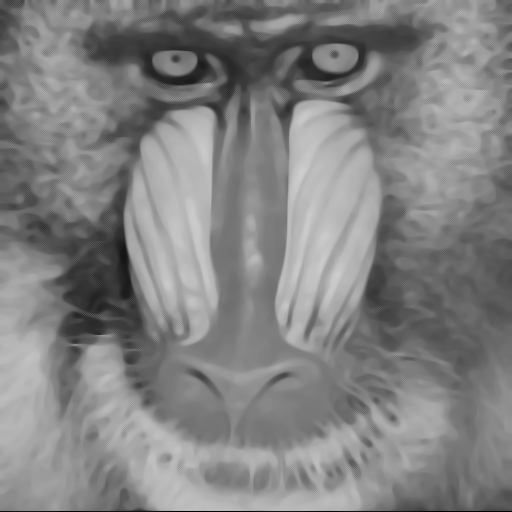
\includegraphics[width=1\textwidth]{../Art/OpenCVITKex1-ans.png} \\
Curvature Flow
\end{center}
\end{columns}
\end{frame}

\subsection{Video Filtering}


\begin{frame}
\frametitle{Basic Video Filtering}
\begin{center}
\begin{itemize}
\item Video filtering is similar to image filtering, except
  \begin{itemize}
  \item use a {\tt VideoCapture} object to read a video file.
  \item loop over each frame in the video and process each one.
  \item display or encode each output frame within the loop.
  \end{itemize}
\end{itemize}
\end{center}
\end{frame}



\begin{frame}
\frametitle{Video Filters}
\begin{itemize}
\item Support video processing natively in ITK
\item Standard framework for multi-frame filters
\item Use ITK's library of image filters in video context
\end{itemize}
\end{frame}


\begin{frame}
\frametitle{More Tutorial Material}
\begin{itemize}
\item  More excercises can be found at:  https://github.com/InsightSoftwareConsortium/ITK-OpenCV-Bridge-Tutorial 
\end{itemize}
\end{frame}






% \section{ITK Video Filters}


\centeredlargetext{white}{black}{
ITK Video Filters
}

%%%%
% Introduction Page
%%%%
\begin{frame}
\frametitle{Introduction}
\begin{itemize}
\item Support video processing natively in ITK
\item Standard framework for multi-frame filters
\item Use ITK's library of image filters in video context
\end{itemize}
\end{frame}


%%%%
% Code walkthrough
%%%%
{
\setbeamertemplate{navigation symbols}{}
\begin{frame}[fragile]
\frametitle{Video Filtering - Median Filter}
\framesubtitle{ITKVideoPipeline/exercise1/ITKVideoSingleFrameFilters.cxx}

\begin{itemize}
\item Video data structure
\lstlistingwithnumber{21}{21}{ITKVideoSingleFrameFilters.cxx}
\pause

\item Video file reader and writer
\item Use OpenCV for video IO
\lstlistingwithnumber{24}{26}{ITKVideoSingleFrameFilters.cxx}
\pause

\item Median image filter
\item Image filter $\rightarrow$ video filter wrapper
\lstlistingwithnumber{22}{23}{ITKVideoSingleFrameFilters.cxx}
\end{itemize}
\end{frame}
}

{
\setbeamertemplate{navigation symbols}{}
\begin{frame}[fragile]
\frametitle{Video Filtering - Median Filter}
\framesubtitle{ITKVideoPipeline/exercise1/ITKVideoSingleFrameFilters.cxx}
\begin{itemize}
\item Types for data structures
\lstlistingwithnumber{36}{39}{ITKVideoSingleFrameFilters.cxx}
\pause

\item Types reader and writer
\lstlistingwithnumber{41}{42}{ITKVideoSingleFrameFilters.cxx}
\pause

\item Types for video median filter
\item Use image filter type to define video filter type
\lstlistingwithnumber{43}{45}{ITKVideoSingleFrameFilters.cxx}
\end{itemize}
\end{frame}
}

{
\setbeamertemplate{navigation symbols}{}
\begin{frame}[fragile]
\frametitle{Video Filtering - Median Filter}
\framesubtitle{ITKVideoPipeline/exercise1/ITKVideoSingleFrameFilters.cxx}
\begin{itemize}
\item Create reader and writer
\lstlistingwithnumber{47}{48}{ITKVideoSingleFrameFilters.cxx}
\pause

\item Create image filter and video median filters
\lstlistingwithnumber{49}{50}{ITKVideoSingleFrameFilters.cxx}
\end{itemize}
\end{frame}
}

{
\setbeamertemplate{navigation symbols}{}
\begin{frame}[fragile]
\frametitle{Video Filtering - Median Filter}
\framesubtitle{ITKVideoPipeline/exercise1/ITKVideoSingleFrameFilters.cxx}
\begin{itemize}
\item Set up reader and writer
\item Tell ITK that we're using OpenCV for IO
\lstlistingwithnumber{52}{54}{ITKVideoSingleFrameFilters.cxx}
\pause

\item Set up radius for (image) median filter
\item Set video filter wrapper to use image median filter internally
\lstlistingwithnumber{56}{60}{ITKVideoSingleFrameFilters.cxx}
\end{itemize}
\end{frame}
}

{
\setbeamertemplate{navigation symbols}{}
\begin{frame}[fragile]
\frametitle{Video Filtering - Median Filter}
\framesubtitle{ITKVideoPipeline/exercise1/ITKVideoSingleFrameFilters.cxx}
\begin{itemize}
\item Connect the pipeline
\item reader $\rightarrow$ videoFilter $\rightarrow$ writer
\lstlistingwithnumber{62}{63}{ITKVideoSingleFrameFilters.cxx}
\pause

\item Try calling Update() to process the entire video
\lstlistingwithnumber{65}{73}{ITKVideoSingleFrameFilters.cxx}
\end{itemize}
\end{frame}
}


%%%%
% Exercise 1
%%%%
{
\setbeamertemplate{navigation symbols}{}
\begin{frame}[fragile]
\frametitle{Exercise 1}
\framesubtitle{Replace median filter with curvature flow filter}
\begin{itemize}
\item Hint 1: Curvature Flow requires {\tt float} as the pixel
  type for output.
\pause

\item Hint 2: OpenCV uses ffmpeg which requires {\tt unsigned char}
  as the pixel type for writing.
\pause

\item Hint 3: Curvature Flow does not take a radius parameter. It's
  salient functions are:
\lstlistingwithnumber{70}{71}{ITKVideoSingleFrameFiltersAnswer.cxx}
\pause

\item Hint 4: To use an image filter in a video pipeline use
  {\tt ImageFilterToVideoFilterWrapper}
\end{itemize}
\end{frame}
}

{
\setbeamertemplate{navigation symbols}{}
\begin{frame}[fragile]
\frametitle{Exercise 1: Answer}
\framesubtitle{Replace median filter with curvature flow filter}
\begin{itemize}
\item Include curvature and cast image filters
\lstlistingwithnumber{22}{23}{ITKVideoSingleFrameFiltersAnswer.cxx}
\pause

\item Re-define types using seperate IO and Real pixel types
\lstlistingwithnumber{37}{43}{ITKVideoSingleFrameFiltersAnswer.cxx}
\end{itemize}
\end{frame}
}

{
\setbeamertemplate{navigation symbols}{}
\begin{frame}[fragile]
\frametitle{Exercise 1: Answer}
\framesubtitle{Replace median filter with curvature flow filter}
\begin{itemize}
\item Define cast filter to convert from Real to IO pixel type
\lstlistingwithnumber{47}{50}{ITKVideoSingleFrameFiltersAnswer.cxx}
\pause

\item Replace median filter with curvature flow filter
\item Use Real pixel type for output
\lstlistingwithnumber{51}{54}{ITKVideoSingleFrameFiltersAnswer.cxx}
\end{itemize}
\end{frame}
}

{
\setbeamertemplate{navigation symbols}{}
\begin{frame}[fragile]
\frametitle{Exercise 1: Answer}
\framesubtitle{Replace median filter with curvature flow filter}
\begin{itemize}
\item Set up video cast filter
\lstlistingwithnumber{68}{68}{ITKVideoSingleFrameFiltersAnswer.cxx}
\pause

\item Set up curvature flow filter
\lstlistingwithnumber{70}{72}{ITKVideoSingleFrameFiltersAnswer.cxx}
\pause

\item Connect the pipeline
\item reader $\rightarrow$ curvature
  flow $\rightarrow$ output caster $\rightarrow$ writer
\lstlistingwithnumber{74}{76}{ITKVideoSingleFrameFiltersAnswer.cxx}
\end{itemize}
\end{frame}
}

{
\setbeamertemplate{navigation symbols}{}
\begin{frame}[fragile]
\frametitle{Running the Example}
\framesubtitle{/home/tutorial/bin/ITK-OpenCV-Bridge-Tutorial/Exercises/ITKVideoPipeline}
\begin{itemize}
\item Run the example with the following command
\begin{verbatim}
      ./exercise1/ITKVideoSingleFrameFilters \
      ~/data/Walk1_short.avi                 \
      ./Walk1_short_median.avi 
\end{verbatim}
\end{itemize}
\end{frame}
}


%%%%
% Exercise 2
%%%%
{
\setbeamertemplate{navigation symbols}{}
\begin{frame}[fragile]
\frametitle{Exercise 2}
\framesubtitle{Compute frame differences after diffusion}
\begin{itemize}
\item Start with solution to Exercise 1 (ITKVideoMultiFrameFilters.cxx)
\pause

\item Hint 1: Use FrameDifferenceVideoFilter
\pause

\item Hint 2: Difference filter's important parameter is:
\lstlistingwithnumber{73}{73}{ITKVideoMultiFrameFiltersAnswer.cxx}
\item This sets the spacing of the frames to be differenced. Setting
  it to 1 means adjacent frames will be used.
\end{itemize}
\end{frame}
}

{
\setbeamertemplate{navigation symbols}{}
\begin{frame}[fragile]
\frametitle{Exercise 2: Answer}
\framesubtitle{Compute frame differences after diffusion}
\begin{itemize}
\item Include frame difference filter
\lstlistingwithnumber{25}{25}{ITKVideoMultiFrameFiltersAnswer.cxx}
\pause

\item Define type for frame difference filter
\item Since this is a native video filter, no wrapper is necessary
\lstlistingwithnumber{57}{58}{ITKVideoMultiFrameFiltersAnswer.cxx}
\pause

\item Create frame difference filter
\lstlistingwithnumber{66}{67}{ITKVideoMultiFrameFiltersAnswer.cxx}
\end{itemize}
\end{frame}
}

{
\setbeamertemplate{navigation symbols}{}
\begin{frame}[fragile]
\frametitle{Exercise 2: Answer}
\framesubtitle{Compute frame differences after diffusion}
\begin{itemize}
\item Set the frame offset to 1
\lstlistingwithnumber{73}{73}{ITKVideoMultiFrameFiltersAnswer.cxx}
\pause

\item Connect the pipeline
\item reader $\rightarrow$ curvature flow $\rightarrow$ output caster
  $\rightarrow$ frame differ $\rightarrow$ writer
\lstlistingwithnumber{81}{84}{ITKVideoMultiFrameFiltersAnswer.cxx}
\end{itemize}
\end{frame}
}

{
\setbeamertemplate{navigation symbols}{}
\begin{frame}[fragile]
\frametitle{Running the Answer}
\framesubtitle{/home/tutorial/bin/ITK-OpenCV-Bridge-Tutorial/Exercises/ITKVideoPipeline}
\begin{itemize}
\item Run the example with the following command
\begin{verbatim}
      ./exercise2/ITKVideoMultiFrameFiltersAnswer \
      ~/data/Walk1_short.avi                      \
      ./Walk1_short_diff.avi 
\end{verbatim}

\item Extra Credit: Add a threshold to the difference output to supress
  background noise
\item {\footnotesize ITKVideoPipeline/exercise1/ITKVideoMultiFrameFiltersAnswer2.cxx}
\end{itemize}
\end{frame}
}


\begin{frame}
\frametitle{Wrap-up}
\begin{itemize}
  \item Send us feedback (good or bad)
  \begin{itemize}
    \item \url{arnaud_gelas@hms.harvard.edu} 
    \item \url{kishore_mosaliganti@hms.harvard.edu} 
    \item \url{sean_megason@hms.harvard.edu}
  \end{itemize}
%   \item Raffle\\
% \includegraphics[height=1.5in]{asus}
\end{itemize}
\end{frame}



\section{Registration}

{
\setbeamertemplate{background}{}
\setbeamertemplate{navigation symbols}{}
\setbeamercolor{background canvas}{bg={black}}
\color{white}
\begin{frame}[plain]
\fontsize{36pt}{36pt}\selectfont
\center
\begin{center}
Refactored Registration Framework
\end{center}

\fontsize{12pt}{12pt}\selectfont
\begin{center}
Insight Software Consortium
\end{center}
\vskip12pt
\begin{center}
 PICSL @ University of Pennsylvania 
\end{center}
\vskip12pt
\begin{center}
 Brian Avants, Nicholas Tustison, Gang Song, \\ 
Baohua Wu, Michael Stauffer, James C. Gee
\end{center}
\end{frame}
}

\subsection{Introduction}

\begin{frame}
\frametitle{What is registration?}
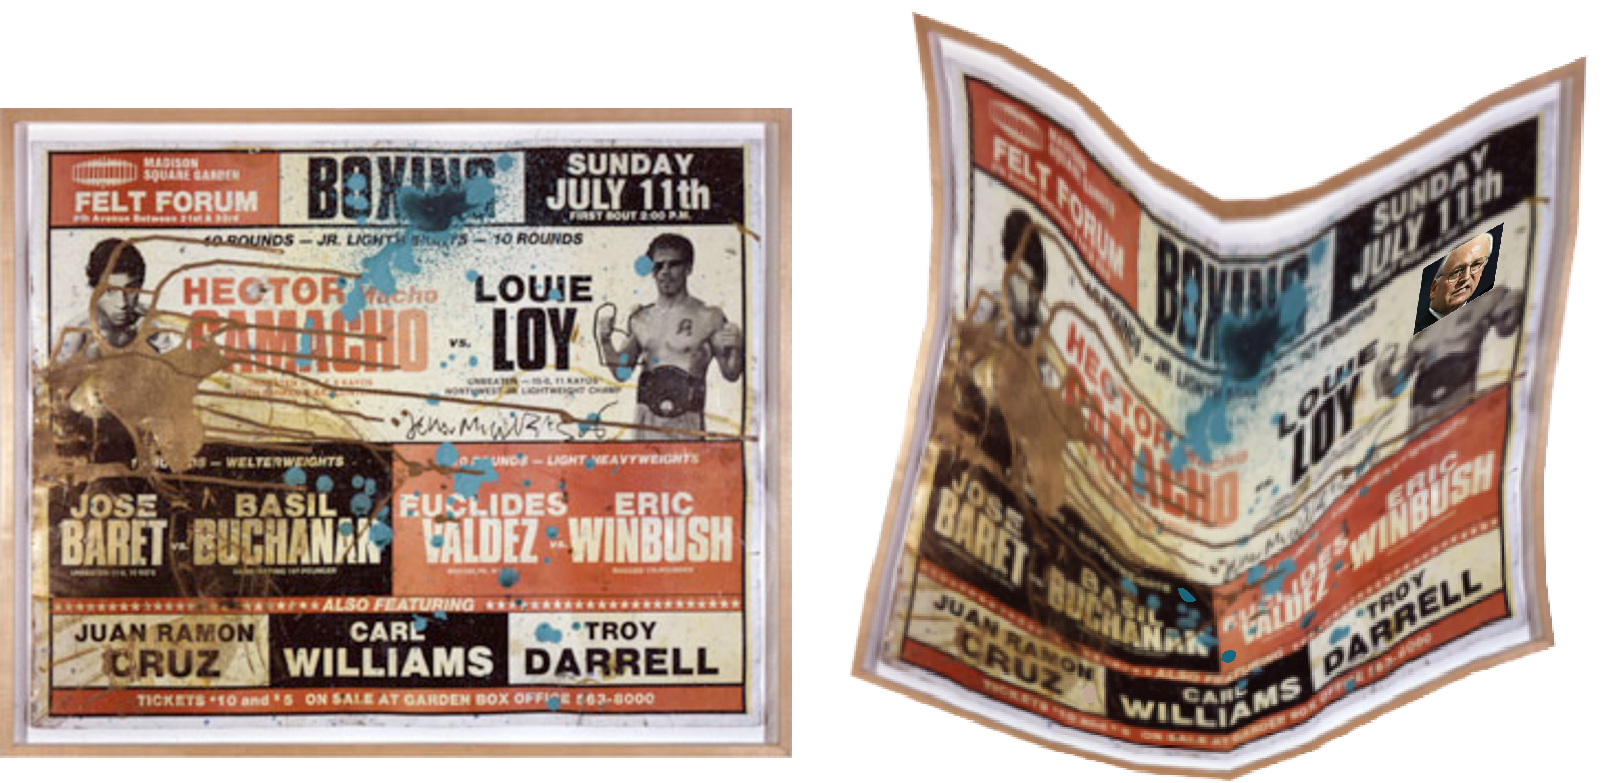
\includegraphics[height=2in]{../Art/RegistrationBasquiatWarp.pdf}
\end{frame}

\begin{frame}
\frametitle{What is registration?}
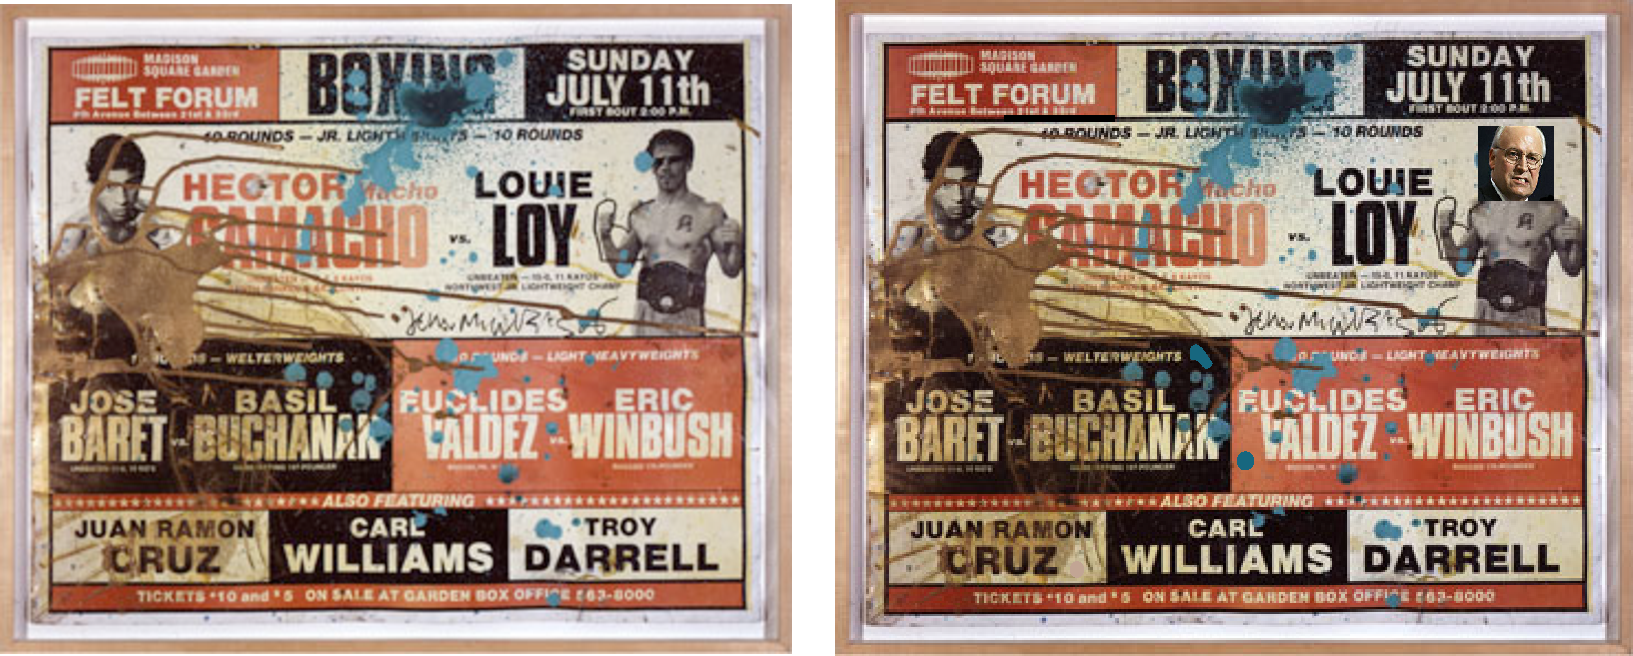
\includegraphics[height=1.8in]{../Art/RegistrationBasquiatDeWarp.pdf}
\vskip20pt
\begin{displaymath}
\| I ( x ) - J(\phi(x)) \|^2  + R(\phi( x))
\end{displaymath}
\end{frame}

 \centeredlargetext{white}{black}{
\centering Enhanced user experience
%
\includegraphics[height=1.8in]{../Art/ITKv4}
 }

 \centeredlargetext{white}{black}{
\centering Unified multi-core framework + parameter-estimation
% 
\includegraphics[height=1.8in]{../Art/ITKv4}
 }


\subsection{Refactoring overview}
\begin{comment}
{

\begin{frame}
\frametitle{Image Registration Refactoring}
\Large
\begin{itemize}
\item Unify frameworks: local \& global 
\pause
\item New metrics and transform operations for vectors \&  tensors
\pause 
\item Composite Transform
\pause
\item Unbiased registration
\pause
\item Multi-threading 
\pause 
\item Automated parameter scaling
\end{itemize}
\end{frame}

\begin{frame}
\frametitle{Unified framework}
\Large
\begin{itemize}
\item Local \& global transforms treated the same in resampler
\item Both types available to (revised) optimizers
\item Revised metrics optimized for these operations
\item Tensors, vector, scalars treated transparently
\end{itemize}
\end{frame}
}
\end{comment}

 \centeredlargetext{white}{black}{
ITK v3 framework
\vskip20pt
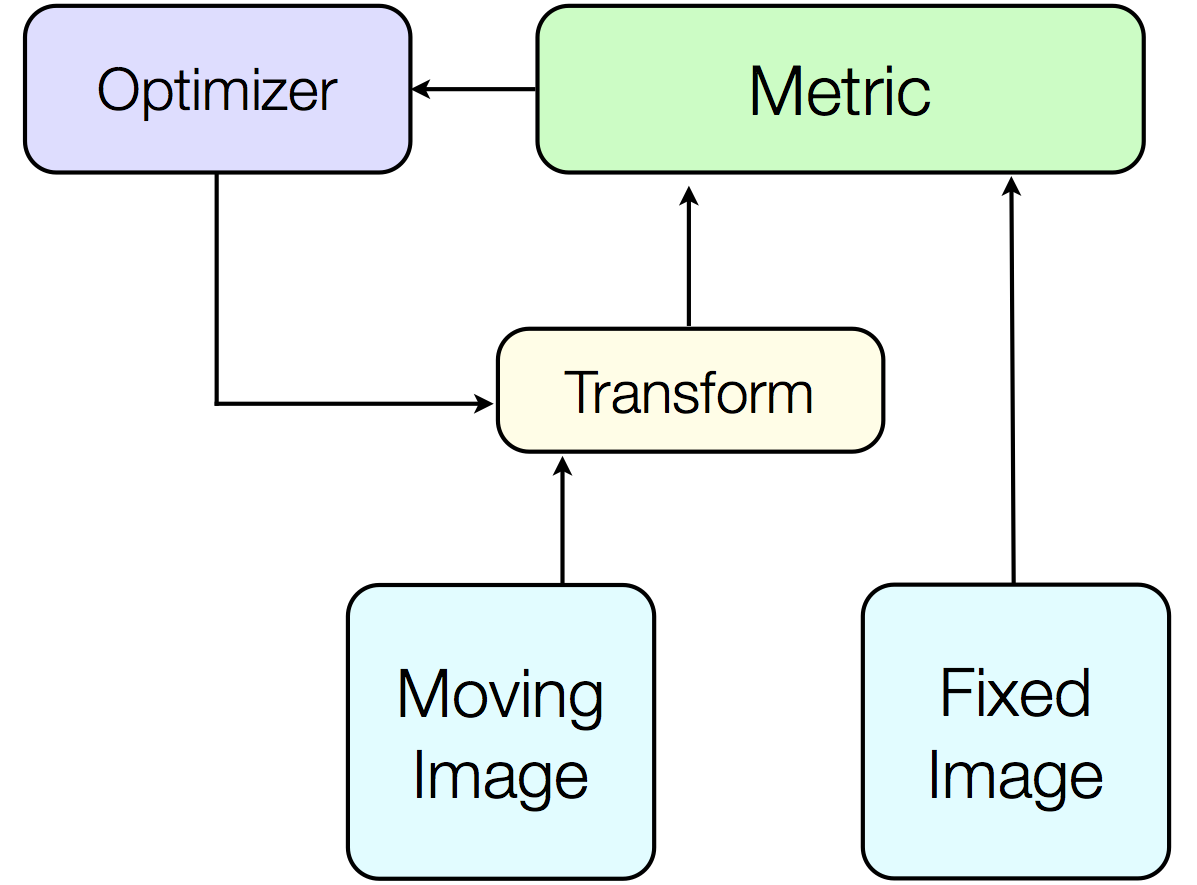
\includegraphics[height=2.2in]{../Art/itkv3reg}
 }

 \centeredlargetext{white}{black}{
ITK v4 framework
\vskip20pt
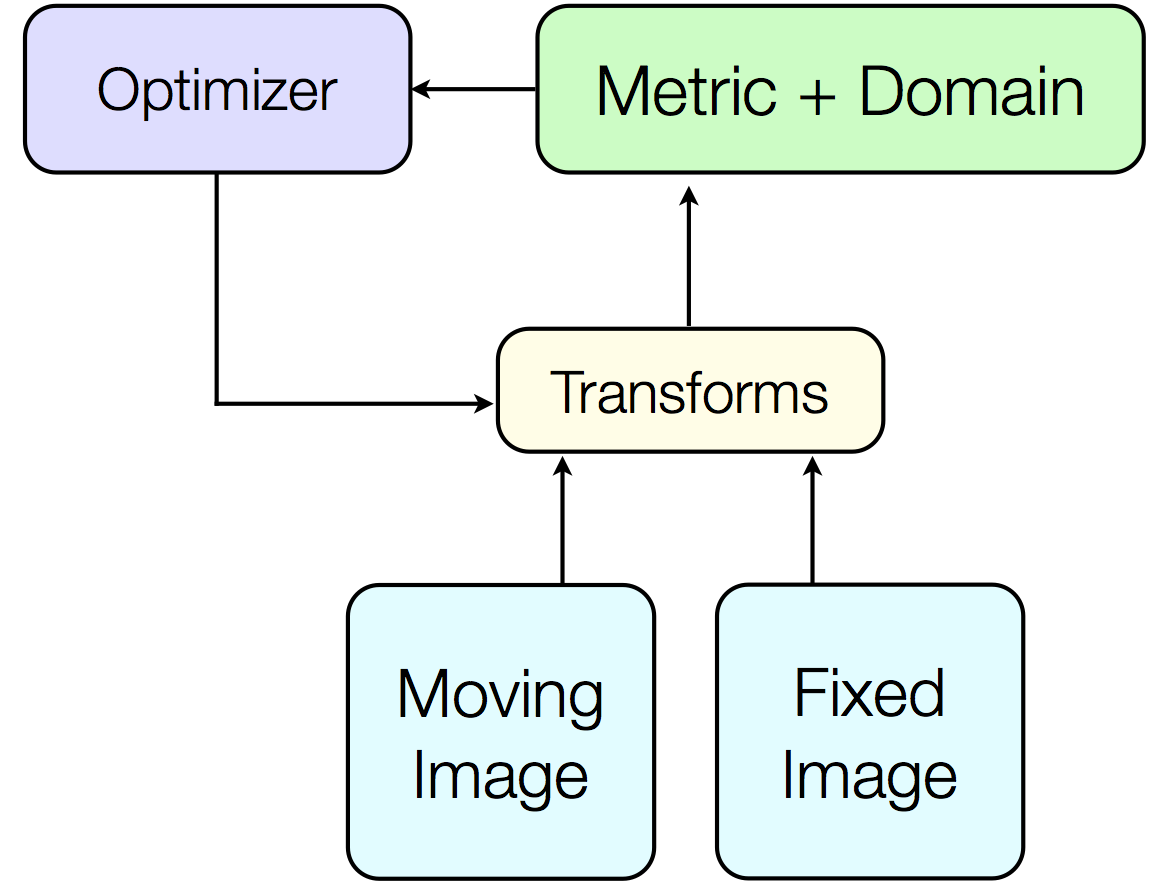
\includegraphics[height=2.2in]{../Art/itkv4reg}
 }

\begin{frame}
\frametitle{Composite transformations}
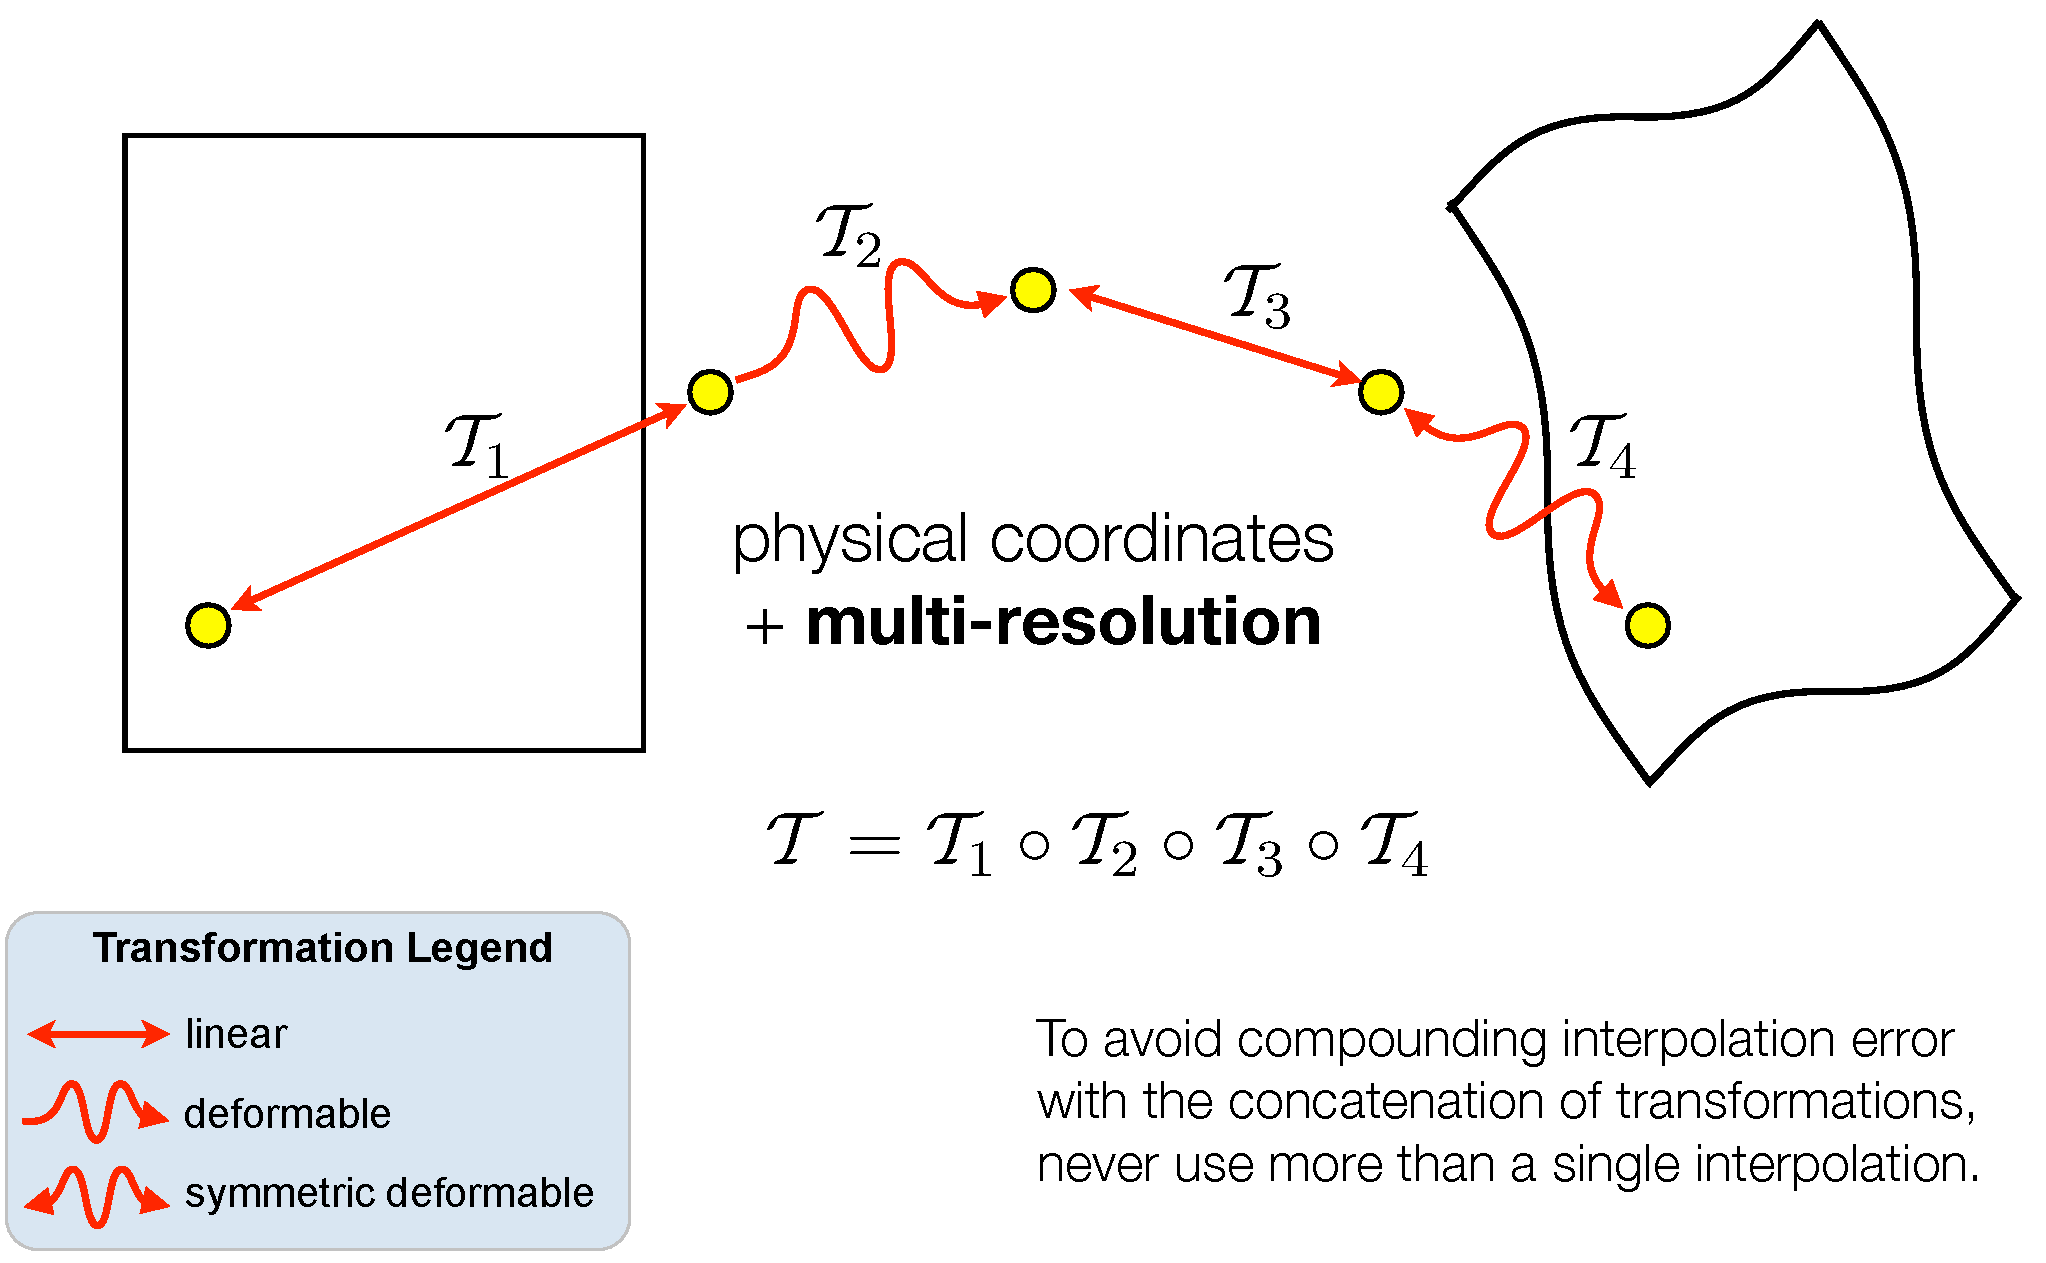
\includegraphics[height=2.5in]{../Art/composite}
\end{frame}

\subsection{Example}
 \centeredlargetext{white}{black}{
\centering Example Registration
}

\begin{frame}
\frametitle{Compile external module}
\begin{itemize}
\item We link the external module
\lstlistingwithnumber{4}{5}{install_registration_code.cxx}
\item We recompile
\lstlistingwithnumber{6}{9}{install_registration_code.cxx}
\item Be sure to compile in Release mode for real applications!
\end{itemize}
\end{frame}


\begin{frame}
\frametitle{Image Registration Refactoring: Brain + N-hood CC}
\textcolor{red}{./bin/ITKRegistrationRefactoringTestDriver itkANTSNeighborhoodCorrelationImageToImageObjectRegistrationTest}\\
\textcolor{blue}{r16slice.jpg r64slice.jpg out.nii.gz  50 500 }\\
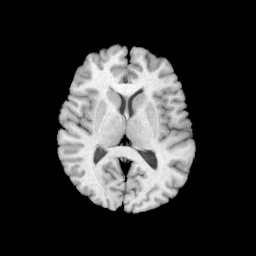
\includegraphics[height=2.2in]{../Art/r16slice.jpg}
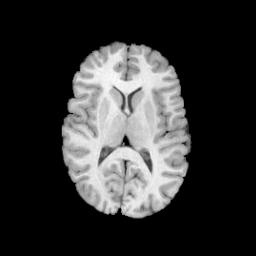
\includegraphics[height=2.2in]{../Art/r64slice.jpg}
\end{frame}

\begin{frame}
\frametitle{Image Registration Code: Brain + N-hood CC}
\begin{itemize}
\item Define the metric
\lstlistingwithnumber{171}{175}{itkANTSNeighborhoodCorrelationImageToImageObjectRegistrationTest.cxx}
\item Define the transforms
\lstlistingwithnumber{165}{168}{itkANTSNeighborhoodCorrelationImageToImageObjectRegistrationTest.cxx}
\lstlistingwithnumber{138}{141}{itkANTSNeighborhoodCorrelationImageToImageObjectRegistrationTest.cxx}
\item Resample the image
\lstlistingwithnumber{201}{202}{itkANTSNeighborhoodCorrelationImageToImageObjectRegistrationTest.cxx}
\end{itemize}

\end{frame}

\begin{frame}
\frametitle{Image Registration Refactoring: Composite Tx + MI}
\textcolor{red}{./bin/ITKRegistrationRefactoringTestDriver itkThevenazMutualInformationImageToImageObjectRegistrationTest }\\
\textcolor{blue}{face\_avg.jpg face\_c.jpg out.nii.gz  50 0.001 0.75 }\\
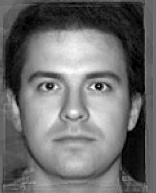
\includegraphics[height=2.2in]{../Art/face_avg.jpg}
\includegraphics[height=2.2in]{../Art/face_c.jpg}
\end{frame}

\begin{frame}
\frametitle{Image Registration Result: Composite Tx + MI}
\textcolor{red}{./bin/ITKRegistrationRefactoringTestDriver itkThevenazMutualInformationImageToImageObjectRegistrationTest }\\
\textcolor{blue}{face\_avg.jpg face\_c.jpg out.nii.gz  50 0.001 0.75 }\\
\includegraphics[height=2.2in]{../Art/face_avg.jpg}
\includegraphics[height=2.2in]{../Art/face_c_to_face_avg.jpg}
\end{frame}

\begin{frame}
\frametitle{Image Registration Code: Composite Tx + MI}
\begin{itemize}
\item Define the metric
\lstlistingwithnumber{186}{189}{itkThevenazMutualInformationImageToImageObjectRegistrationTest.cxx}
\item Estimate scaling parameters for the affine transform
\lstlistingwithnumber{207}{210}{itkThevenazMutualInformationImageToImageObjectRegistrationTest.cxx}
\item Run the affine then add it to composite along with a new
  deformation transform
\lstlistingwithnumber{233}{238}{itkThevenazMutualInformationImageToImageObjectRegistrationTest.cxx}
\end{itemize}
\end{frame}

\begin{frame}
\frametitle{Image Registration Refactoring Example}
\textcolor{red}{./bin/ITKRegistrationRefactoringTestDriver itkThevenazMutualInformationImageToImageObjectRegistrationTest }\\
\textcolor{blue}{face\_avg.jpg face\_b.jpg out.nii.gz  50 0.001 0.75 }\\
\includegraphics[height=2.2in]{../Art/face_avg.jpg}
\includegraphics[height=2.2in]{../Art/face_b.jpg}
\end{frame}

\begin{frame}
\frametitle{Image Registration Refactoring Example}
\textcolor{red}{./bin/ITKRegistrationRefactoringTestDriver itkThevenazMutualInformationImageToImageObjectRegistrationTest }\\
\textcolor{blue}{face\_avg.jpg face\_b.jpg out.nii.gz  50 0.001 0.75 }\\
\includegraphics[height=2.2in]{../Art/face_avg.jpg}
\includegraphics[height=2.2in]{../Art/face_b_to_face_avg_aff.jpg}
\end{frame}
\begin{frame}
\frametitle{Image Registration Refactoring Example}
\textcolor{red}{./bin/ITKRegistrationRefactoringTestDriver itkThevenazMutualInformationImageToImageObjectRegistrationTest }\\
\textcolor{blue}{face\_avg.jpg face\_b.jpg out.nii.gz  50 0.001 0.75 }\\
\includegraphics[height=2.2in]{../Art/face_avg.jpg}
\includegraphics[height=2.2in]{../Art/face_b_to_face_avg.jpg}
\vskip12pt
25 seconds (1 thread) vs 16 seconds (2 threads) on Macbook Air.
\end{frame}

\begin{frame}
\frametitle{Image Registration Refactoring Example}
\textcolor{red}{./bin/ITKRegistrationRefactoringTestDriver itkThevenazMutualInformationImageToImageObjectRegistrationTest }\\
\textcolor{blue}{r16slice.jpg r64slice\_neg.jpg out.nii.gz  50 0.001 0.75 }\\
\includegraphics[height=2.2in]{../Art/r16slice.jpg}
\includegraphics[height=2.2in]{../Art/r64slice_neg.jpg}
\end{frame}

\begin{frame}
\frametitle{Image Registration Refactoring Example}
\textcolor{red}{./bin/ITKRegistrationRefactoringTestDriver itkThevenazMutualInformationImageToImageObjectRegistrationTest }\\
\textcolor{blue}{r16slice.jpg r64slice\_neg.jpg out.nii.gz  50 0.001 0.75 }\\
\includegraphics[height=2.2in]{../Art/r16slice.jpg}
\includegraphics[height=2.2in]{../Art/r64slice_neg_to_16.jpg}
\end{frame}

\subsection{Summary of new features}

\begin{frame}
\frametitle{New metrics}
\Large
\begin{itemize}
\item Metrics produce consistent results across threads.
\item Sparse and dense neighborhood correlation.
\item New mutual information implementation.
\item Point sets ---  euclidean, pse, Jensen-Havrda-Charvat-Tsallis (JHCT).
\item Tensor --- deviatoric and Euclidean.
\item Vector --- arbitrary length (non-geometric) and covariant.
\end{itemize}
\end{frame}

\begin{frame}
\frametitle{New transform models}
\Large
\begin{itemize}
\item As in ITKv3 $+$ some new ones + thread safety 
\item Displacement transforms
\item Updated bspline transforms
\item Poly-affine
\item Diffeomorphic (TBD)
\item Velocityfield --- needs optimizer
\item GPU Demons!!
\end{itemize}
\end{frame}

\begin{frame}
\frametitle{New optimizers}
\Large
\begin{itemize}
\item Multi-threaded update functions
\item Efficient use of parameters for high-dimensional transformations
\item Automated parameter adjustment via Quasi-Newton $+$ moving parameter estimation.
\end{itemize}
\end{frame}

\begin{frame}
\Large
\frametitle{Multi-threading}
\textcolor{red}{ ITK\_GLOBAL\_DEFAULT\_NUMBER\_OF\_THREADS=NT}\\
\textcolor{red}{export ITK\_GLOBAL\_DEFAULT\_NUMBER\_OF\_THREADS}
\vskip20pt
\textcolor{blue}{metric-$>$SetNumberOfThreads(2)}
\includegraphics[height=1.5in]{../Art/cctran}~~\includegraphics[height=1.5in]{../Art/ccfield}
\end{frame}

\subsection{Conclusion}

\begin{frame}
\Large
\frametitle{References relevant to ITKv4 development}
\includegraphics[height=3.2in]{../Art/registration_references}
\end{frame}

\begin{frame}
\Large
\frametitle{Recap \& Conclusion}
\begin{itemize}
\item Local \& global support transforms in same framework
\pause
\item Speed-up on multi-core machines for all high-dimensional metrics ($~N$-cores)
\pause
\item Multivariate and multi-component metrics coming!
\pause
\item Tensors, vector, scalars, landmarks, diffeomorphisms ... 
\pause
\item Evaluation will take some time and could use your help.
\pause
\item Looking forward to getting feedback on insight-users! 
\end{itemize}
\end{frame}


% \section{Statistics Refactoring}


\centeredlargetext{white}{black}{
Statistics Framework
}

{
\setbeamertemplate{background}{}
\begin{frame}
\frametitle{Statistics Refactoring Team - 2007}
\large
\begin{itemize}
\item Brad Davis
\item Andinet Enquobahrie
\item Luis Ibanez
\end{itemize}
\end{frame}
}


{
\setbeamertemplate{background}{}
\begin{frame}
\small
\frametitle{Migration Pages}
\begin{itemize}
\item \url{http://www.itk.org/Wiki/Proposals:Refactoring_Statistics_Framework_2007_Migration_Users_Guide}
\end{itemize}
\end{frame}
}


{
\setbeamertemplate{background}{}
\begin{frame}
\small
\frametitle{Major Changes}
\begin{itemize}
\item Calculators became Filters
\item Samples are now DataObjects
\item Better Traits
\item Better Types (Frequency)
\end{itemize}
\end{frame}
}



% \centeredlargetext{white}{black}{
FEM Refactoring
}

\begin{frame}
\frametitle{FEM Refactoring}
\Huge
\begin{itemize}
\item Code Clean up
\pause
\item Removed subversive pointers
\pause
\item FEM IO
\end{itemize}
\end{frame}



\section{Brief overview of other improvements}

\section{SimpleITK}

\centeredlargetext{white}{black}{
SimpleITK
}


{
\setbeamertemplate{background}{}
\begin{frame}
\frametitle{SimpleITK}
\Huge
\begin{itemize}
\item Hiding Templates
\pause
\item Smarter IO
\pause
\item Procedural Programming
\pause
\item Easier Wrapping
\pause
\item Binary Distribution
\pause
\item See SimpleITK Tutorial\dots
\end{itemize}
\end{frame}
}




\centeredlargetext{black}{white}{
New Fields
}

\include{NewFields}


\centeredlargetext{white}{black}{
Video Bridge
}


\begin{frame}
\frametitle{Video Bridge}
\Huge
\begin{itemize}
\item OpenCV
\pause
\item VXL
\pause
\item Video Filters
\end{itemize}
\end{frame}


\centeredlargetext{white}{black}{
Video Grabber
}


\begin{frame}
\frametitle{Video Grabber}
\Huge
\begin{itemize}
\item Laparoscopy
\pause
\item Ultrasound
\end{itemize}
\end{frame}


\centeredlargetext{white}{black}{
Microscopy
}


\begin{frame}
\frametitle{Microscopy}
\Huge
\begin{itemize}
\item Deconvolution
\pause
\item Denoising
\pause
\item Color correction
\pause
\item Colocalization
\pause
\item File Formats
\end{itemize}
\end{frame}


\centeredlargetext{black}{white}{
Large Images
}


\begin{frame}
\frametitle{Large Images}
\Huge
\begin{itemize}
\item JPEG 2000
\pause
\item Tiling
\pause
\item HDF5
\pause
\item Multi-Resolution Levels
\end{itemize}
\end{frame}


\centeredlargetext{black}{white}{
Insight Journal
}

\begin{frame}
\frametitle{Insight Journal}
\Huge
\begin{itemize}
\item Git Backend
\pause
\item Virtual Appliances
\pause
\item CDE
\pause
\item Reproducible Research
\end{itemize}
\end{frame}


\centeredlargetext{black}{white}{
Migration Guide
}


\centeredlargetext{white}{black}{
\url{http://itk.org/migrationv4}
}


\centeredlargetext{white}{black}{
Live Long\\
and\\
Prosper !
}


\end{document}
